\documentclass[spanish,12pt,a4paper, openright, titlepage, onecolumn, twoside]{book}
\usepackage[spanish]{babel}
\usepackage[latin1]{inputenc}
\usepackage[final]{graphicx}
\usepackage[]{color}
\graphicspath{{./figuras/}}

%%*----------------------------------------------------------------------*
%|                                                                      |
%| File Name            : Gant_Chart.tex                                |
%| Create Date          : June 15th, 2008                               |
%| Last Modification    : June 03rd, 2008                               |
%| Author               : PSTricks Page                                 |
%|                                                                      |
%*----------------------------------------------------------------------*
\usepackage{lscape}
\usepackage{pstricks}
\usepackage{pst-grad}
\usepackage{pst-xkey}
\usepackage{multido}

\makeatletter

% "pspicture" environment or not?
\newif\ifPst@PstPicture
\define@key[psset]{}{PstPicture}[true]{\@nameuse{Pst@PstPicture#1}}
% Intervals to show?
\newif\ifPst@GanttChartShowIntervals
\define@key[psset]{}{ChartShowIntervals}[true]{\@nameuse{Pst@GanttChartShowIntervals#1}}
% Style for the tasks
\define@key[psset]{}{TaskStyle}{\def\psk@GanttTaskStyle{#1}}
% Which line (for multiple tasks in one line)
\newif\ifPst@GanttSameLine
\define@key[psset]{}{SameLine}[true]{\@nameuse{Pst@GanttSameLine#1}}
% Name for unit interval
\define@key[psset]{}{ChartUnitIntervalName}{\def\psk@GanttChartUnitIntervalName{#1}}
% Name for basic unit
\define@key[psset]{}{ChartUnitBasicIntervalName}{\def\psk@GanttChartUnitBasicIntervalName{#1}}
% Unit interval for the tasks (7 for a week, 30 for a month, etc.)
% Warning: define it before "TaskUnitType"!
\define@key[psset]{}{TaskUnitIntervalValue}{%
    \pst@cntg=#1\relax
    \edef\psk@GanttTaskUnitIntervalValue{\the\pst@cntg}}
% Unit type for the tasks (UnitIntervalName or UnitBasicIntervalName)
\define@key[psset]{}{TaskUnitType}{%
    \edef\psk@GanttTaskUnitValue{#1}%
    % Validation of the parameter
    \ifx\psk@GanttTaskUnitValue\psk@GanttChartUnitIntervalName
	\edef\psk@GanttTaskUnitValue{\psk@GanttTaskUnitIntervalValue}%
    \else
	\ifx\psk@GanttTaskUnitValue\psk@GanttChartUnitBasicIntervalName
	    \def\psk@GanttTaskUnitValue{1}%
	\else
	    {\@pstrickserr{GanttTaskUnitType must be `\psk@GanttChartUnitIntervalName'
                   or `\psk@GanttChartUnitBasicIntervalName'
                  (and not `\psk@GanttTaskUnitValue')}\@eha}%
	\fi
    \fi%
}
% Outside label for the tasks
\define@key[psset]{}{TaskOutsideLabel}{\def\psk@GanttTaskOutsideLabel{#1}}
% Inside label for the tasks
\define@key[psset]{}{TaskInsideLabel}{\def\psk@GanttTaskInsideLabel{#1}}
% Maximum outside size label for the tasks (in unit TaskUnitType !)
\define@key[psset]{}{TaskOutsideLabelMaxSize}{%
    \pst@cntg=#1\relax
    \edef\psk@GanttTaskOutsideLabelMaxSize{\the\pst@cntg}}

% Default values
% --------------
% pspicture environment, don't show intervals, default task style,
% unit for tasks is a week (so 7 days), no outside and inside labels
\psset{%
    PstPicture=true,ChartShowIntervals=false,TaskStyle=TaskStyleDefault,
    ChartUnitIntervalName=Week,ChartUnitBasicIntervalName=Day,
    TaskUnitIntervalValue=7,TaskUnitType=Week,SameLine=false,
    TaskOutsideLabel=,TaskInsideLabel=,TaskOutsideLabelMaxSize=0}

\newpsstyle{TaskStyleDefault}{fillstyle=solid,fillcolor=yellow}

% The environment \PstGanttChart
% ------------------------------

% Syntax: \PstGanttChart[parameters]{Number of tasks}{Number of days}
\def\PstGanttChart{\@ifnextchar[\PstGanttChart@i{\PstGanttChart@i[]}}

\def\PstGanttChart@i[#1]#2#3{%
\pst@GanttTaskCnt=\z@  % hv we need it to be reset
\begingroup
\psset{unit=0.1,#1}    % Affectation of local parameters
%
\ifPst@PstPicture               % "pspicture" environment
  \pst@cnta=\psk@GanttTaskOutsideLabelMaxSize
  \multiply\pst@cnta\psk@GanttTaskUnitValue
  %
  \pst@cntb=#2
  \multiply\pst@cntb by 5
  \advance\pst@cntb\@ne
  %
  \pst@cntc=#3
  \multiply\pst@cntc\psk@GanttTaskUnitValue
  \advance\pst@cntc\tw@
  %
  \ifPst@GanttChartShowIntervals
    \pspicture(-\pst@cnta,-\pst@cntb)(\pst@cntc,2)
  \else
    \pspicture(-\pst@cnta,-\pst@cntb)(\pst@cntc,0)
  \fi
\fi
\psframe(0,-\pst@cntb)(\pst@cntc,0)
%
\ifPst@GanttChartShowIntervals
  % We will show the intervals
  \pst@cnta=#3
  \multiply\pst@cnta\psk@GanttTaskUnitValue
  \divide\pst@cnta\psk@GanttTaskUnitIntervalValue
  \advance\pst@cnta\@ne
  %
  \pst@cntb=#2
  \multiply\pst@cntb by 5
  \advance\pst@cntb\@ne
  %
  \pst@dima=\psk@GanttTaskUnitIntervalValue pt
  \divide\pst@dima\tw@
  \advance\pst@dima\@ne pt
  \pst@dimtonum{\pst@dima}{\pst@tempa}
  %
  \multido{\iInterval=1+1,\iIntervalPos=1+\psk@GanttTaskUnitIntervalValue,
           \nIntervalPos=\pst@tempa+\psk@GanttTaskUnitIntervalValue.0}{\pst@cnta}{%
    \ifnum\iInterval=\pst@cnta
      \psline(\iIntervalPos,0)(\iIntervalPos,1.5)
      \psline[linestyle=dotted](\iIntervalPos,-\pst@cntb)(\iIntervalPos,0)
    \else
      \rput(\nIntervalPos,1){\psk@GanttChartUnitIntervalName\space\iInterval}
      \psline(\iIntervalPos,0)(\iIntervalPos,1.5)
      \psline[linestyle=dotted](\iIntervalPos,-\pst@cntb)(\iIntervalPos,0)
    \fi}
\fi}

\def\endPstGanttChart{%
\ifPst@PstPicture
  \endpspicture                 % End of "pspicture" environment
\fi
\endgroup%
}

% The macro \PstGanttTask
% -----------------------

\newcount\pst@GanttTaskCnt
\pst@GanttTaskCnt=\z@

% Syntax: \PstGanttTask[parameters]{Start}{Length}
\def\PstGanttTask{\@ifnextchar[\PstGanttTask@i{\PstGanttTask@i[]}}

\def\PstGanttTask@i[#1]#2#3{%
\advance\pst@GanttTaskCnt\m@ne
\begingroup
\psset{#1}%            % Affectation of local parameters
\ifPst@GanttSameLine
  \global\advance\pst@GanttTaskCnt\@ne
\fi
% Frame
\pst@cnta=\psk@GanttTaskUnitValue
\multiply\pst@cnta by #2
\advance\pst@cnta\@ne
%
\pst@cntb=\psk@GanttTaskUnitValue
\multiply\pst@cntb by #3
\advance\pst@cntb\pst@cnta
%
\pst@cntc=\pst@GanttTaskCnt
\multiply\pst@cntc by 5
%
\pst@cntd=\pst@cntc
\advance\pst@cntd by 4
%
\psframe[style=\psk@GanttTaskStyle](\pst@cnta,\pst@cntc)(\pst@cntb,\pst@cntd)
% Inside label
\ifx\psk@GanttTaskInsideLabel\empty
\else
  \pst@dima=\pst@cnta pt
  \advance\pst@dima\pst@cntb pt
  \divide\pst@dima\tw@
  \pst@dimtonum{\pst@dima}{\pst@tempa}
  %
  \pst@dimb=\pst@cntc pt
  \advance\pst@dimb\pst@cntd pt
  \divide\pst@dimb\tw@
  \pst@dimtonum{\pst@dimb}{\pst@tempb}
  %
  \rput(\pst@tempa,\pst@tempb){\psk@GanttTaskInsideLabel}
\fi
% Outside label
\ifx\psk@GanttTaskOutsideLabel\empty
\else
  \pst@dimb=\pst@cntc pt
  \advance\pst@dimb\pst@cntd pt
  \divide\pst@dimb\tw@
  \pst@dimtonum{\pst@dimb}{\pst@tempb}
  \rput[r](-1.5,\pst@tempb){\psk@GanttTaskOutsideLabel}
\fi
\endgroup% Affectation of local parameters
}

\makeatother




%\usepackage{pstricks}
%\usepackage{pst-gantt}
%\usepackage{pstricks-add}
\newcommand{\p}{{\paragraph}}
\usepackage{pgfgantt}
\usepackage{lscape}

%Avoid orphans
\widowpenalty=300
\clubpenalty=300


\begin{document}
\frontmatter
%Evitar que llame a las tablas cuadros.
\renewcommand{\tablename}{Tabla}
\renewcommand{\listtablename}{�ndice de tablas}

\begin{titlepage}
\thispagestyle{empty}
\begin{center}


\includegraphics[width=0.4\textwidth]{./logo}\\[1cm] 

\textsc{\large\textbf{UNIVERSIDAD DE CASTILLA-LA MANCHA}}\\[0.5cm]

\textsc{\large{\textbf{ESCUELA SUPERIOR DE INGENIER�A INFORM�TICA}}}\\[0.4cm]

\hrule  \hspace*{\fill} \\[0.4cm]

\textsc{\large\textbf{M�STER UNIVERSITARIO EN TECNOLOG�AS INFORM�TICAS AVANZADAS} } \\[0.8cm]
\textsc{\Large\textbf{TRABAJO FIN DE M�STER}}\\[0.3cm]
\hrule  \hspace*{\fill} \\[1.0cm]

\textsc{\huge\textbf{�Aceleraci�n de software de an�lisis de genoma mediante paralelismo?}}\\[2.0cm]

\textsc{\LARGE\textbf{Ra�l Moreno Gald�n}}\\[2.0cm]


\begin{flushright}
\vfill
\textsc{\large\textbf{\today}}
\end{flushright}

\end{center}

\newpage
\thispagestyle{empty}

\begin{center}


\includegraphics[width=0.4\textwidth]{./logo}\\[1cm] 

\textsc{\large \textbf{UNIVERSIDAD DE CASTILLA-LA MANCHA}}\\[0.5cm]

\textsc{\large \textbf{ESCUELA SUPERIOR DE INGENIER�A INFORM�TICA}}\\[0.4cm]

\hrule  \hspace*{\fill} \\[0.4cm]

\textsc{\Large \textbf{Departamento de Sistemas Inform�ticos} } \\[0.8cm]
\textsc{\Large \textbf{TRABAJO FIN DE M�STER}}\\[0.3cm]
\hrule  \hspace*{\fill} \\[1.0cm]

\textsc{\huge \textbf{�Aceleraci�n de software de an�lisis de genoma mediante paralelismo?}}\\[2.0cm]


\begin{flushleft}
\begin{tabular}{ l l }
\textsc{\Large \textbf{Autor:}}	& \textsc{\Large \textbf{Ra�l Moreno Gald�n}}\\[0.3cm]
\textsc{\Large \textbf{Director:}}	& \textsc{\Large \textbf{Dr. Diego Cazorla Lopez}}\\[0.3cm]
\textsc{\Large \textbf{Codirector:}}	& \textsc{\Large \textbf{Dr. Enrique Arias Antunez}}\\[0.3cm]
\end{tabular}
\end{flushleft}

\begin{flushright}
\vfill
\textsc{\large\textbf{\today}}
\end{flushright}

\end{center}

\end{titlepage}


%\begin{flushleft}
%
%\emph{\large{Autor:}} 
%\newline
%\newline
%\LARGE{Ra�l Moreno Gald�n} 
%\newline
%\newline
%\normalsize\texttt{raulmorenogaldon@gmail.com} \\
%
%%\author{Ra�l Moreno Gald�n\\
%%	UCLM\\\\
%%	\texttt{raulmorenogaldon@gmail.com}}
%%\date{\today}
%\end{flushleft}

%no numerar esta pagina
\thispagestyle{empty}
\section*{}
\newpage
\thispagestyle{empty}

\vspace{10cm}
\begin{flushright}\textbf{\Large A tal tal tal}\end{flushright}{\Large \par}

\newpage

\thispagestyle{empty}

\chapter*{Agradecimientos}

asdfasdfasdfasd

\begin{flushright}\emph{Ra�l Moreno Gald�n.} Albacete, Espa�a, Junio 2013.\end{flushright}


\chapter*{Resumen}
adsfasfasfdas


%\thispagestyle{empty}
\tableofcontents

\newpage

\listoffigures{}
\listoftables{}

\setcounter{secnumdepth}{2}

%intentar no romper palabras
\sloppy
\mainmatter
\chapter{Introducci�n}

Este capitulo trata de ofrecer una visi�n general sobre la linea de investigaci�n que se quiere seguir durante la realizaci�n de esta tesis doctoral y cuales son las motivaciones que la impulsan. Adem�s se presenta un breve resumen sobre la estructura que sigue esta memoria para orientar al lector sobre sus contenidos.\\

\section{Motivaci�n}

El ADN \cite{molecularbio,humangenomeweb} (�cido desoxirribonucleico) de todos los organismos vivos conocidos contiene las instrucciones gen�ticas usadas en su desarrollo y funcionamiento, es como una plantilla de la que saldr� el organismo final. El papel de la mol�cula de ADN es el de almacenar a largo plazo informaci�n sobre esa plantilla, plano o receta, como quiera llamarse, que al fin y al cabo es un \textit{c�digo}. Este c�digo contiene las instrucciones necesarias para construir los componentes de las c�lulas (prote�nas y mol�culas de ARN \cite{molecularbio,humangenomeweb} o �cido ribonucleico) y adem�s se transmite de generaci�n en generaci�n.\\

Un gen \cite{molecularbio,humangenomeweb} es una regi�n de ADN que influye en una caracter�stica particular de un organismo (color de los ojos por ejemplo). Estos genes son el plano para producir las prote�nas, que regulan las funciones del organismo. Si un gen resultase cambiado se podr�a producir una falta de prote�nas dando lugar a enfermedades. En otros casos podr�a producir efectos beneficiosos que generar�an individuos m�s adaptados a su entorno (en esto se basa la evoluci�n).\\

La b�squeda del estudio de la estructura del ADN permite por tanto el desarrollo de multitud de herramientas tecnol�gicas que explotan sus propiedades para analizar su implicaci�n en problemas concretos. Por ejem\-plo la carac\-terizaci�n de la variabilidad individual de un paciente en respuesta a un determinado f�rmaco, o la obtenci�n de una caracter�stica com�n de un grupo de individuos de inter�s. Los beneficios son visibles en medicina, pero tambi�n en agricultura y ganader�a (obtener carnes y cultivos de m�s calidad). Es posible incluso determinar la evoluci�n que ha seguido una especie analizando las mutaciones \cite{molecularbio} que ha sufrido su ADN y que quedan grabadas en el mismo, avanzando en el campo de la ecolog�a y la antropolog�a.\\

En cuanto a la \textit{bioinform�tica} son muchos los avances que se han realizado en los �ltimos a�os en el campo de la gen�mica. La tecnolog�a de secuenciaci�n \cite{generationsseq} cada vez produce m�s datos a una escala sin precedentes, lo cual hace surgir dificultades a la hora de almacenar y procesar esos datos. Estos datos necesitan de recursos computacionales y t�cnicas de procesamiento que permitan obtener resultados r�pidamente, permitiendo avanzar a los campos cient�ficos que se basan en los mismos.\\

Se han desarrollado muchas soluciones en los �ltimos a�os destinadas al an�lisis del ADN, pero ninguna ha conseguido una alta calidad y completitud. Los principales problemas encontrados son:
\begin{itemize}
\item
Normalmente solo resuelven una parte espec�fica del an�lisis y fallan en otras funciones, lo que provoca el uso de diferentes programas a modo \textit{pipeline}.
\item
Implementaciones pobres, con bugs y rendimiento muy bajo en t�rminos de tiempo de ejecuci�n y necesidades de memoria.
\item
No est�n preparadas para dar el salto a distintos escenarios de computaci�n paralela como puede ser un \textit{cluster} con varios elementos de procesamiento interconectados entre s�.
\item
Falta de documentaci�n.
\end{itemize}
Estos inconvenientes se convierten en un cuello de botella cuando los precios de los recursos de c�mputo bajan mientras que los datos a procesar se incrementan.\\

Lo que se busca por tanto en esta \textit{tesis} es la elaboraci�n de un conjunto de programas que permitan analizar estos datos masivos obtenidos por los secuenciadores de ADN, que exploten al m�ximo las plataformas de computaci�n de las que se puedan disponer y por tanto acelerar no solo la caracterizaci�n de un ADN, sino las ciencias que se apoyan en el mismo. Para acelerar estos programas se puede hacer uso de la programaci�n paralela, la cual permite utilizar var�as m�quinas simult�neamente para obtener resultados. Adem�s ser� necesario contar con mecanismos de gesti�n y tratamiento de grandes cantidades de datos para poder manejar los que producen los secuenciadores.\\

\section{Estructura de la memoria}

?????\\
\chapter{Asignaturas Cursadas}

En este cap�tulo se resumen las asignaturas elegidas por el alumno para su realizaci�n durante el m�ster, sus objetivos y contenidos.\\
En general, las asignaturas tienen como objetivo general la formaci�n del personal investigador en un amplio espectro, desde la formaci�n en t�rminos t�cnicos de inform�tica a aspectos que lo relacionan con el �mbito investigador.\\
Se presentar� el trabajo realizado en cada una de la asignaturas cursadas, su metodolog�a. y cu�l es su relaci�n con el tema de investigaci�n de la Tesis.\\

\section[Generaci�n de documentos cient�ficos]{Generaci�n de documentos cient�ficos en inform�tica}

\subsection{Descripci�n}

Esta asignatura engloba varios aspectos del mundo de la investigaci�n, como son la elaboraci�n de publicaciones, de documentos cient�ficos y de an�lisis de propiedades de los entornos a investigar.\\

La primera parte del curso trata de introducir al alumno en el mundo de la investigaci�n, present�ndole a qu� se va a enfrentar y c�mo se eval�an los trabajos cient�ficos mediante publicaciones y en qu� lugares, tanto a nivel de investigador como a nivel de organizaci�n.\\

La segunda parte se centra en la elaboraci�n de documentos cient�ficos, c�mo deben organizarse y escribirse para que sean aceptados en el �mbito investigador. Adem�s, se presentan algunas herramientas, entre ellas \LaTeX, que permiten escribir documentos de forma limpia y adecuada.\\

En la �ltima parte del curso se ense�a al alumno a organizar sus experimentos respetando ciertas condiciones. Esto permite realizar posteriormente contrastes sobre los resultados de los mismos para obtener finalmente conclusiones fiables y s�lidas.\\

\subsection{Trabajo realizado}

En la primera parte de la asignatura se realizan trabajos de b�squeda de informaci�n, a modo de entrenamiento, sobre plataformas dedicadas a este tipo de b�squedas, entre las cuales se encuentran Google Scholar, Scopus y Web of knowledge. Uno de los objetivos de este trabajo es realizar un an�lisis de la calidad de los profesores del Departamento de Sistemas Inform�ticos de la ESII en Albacete, utilizando como m�trica los �ndices H.\\

Para la segunda parte de la asignatura se realizan diversos ejercicios de entrenamiento en el uso de \LaTeX. El objetivo de estos ejercicios es la preparaci�n para poder realizar finalmente la parte escrita y la presentaci�n del trabajo final de la asignatura mediante esta herramienta.\\

En la �ltima parte de la asignatura se ense�a al alumno a realizar contrastes de hip�tesis, sobre datos obtenidos de experimentos mediante la realizaci�n de ejercicios de entrenamiento. Esto permite obtener propiedades importantes acerca de esos datos.\\

Para el trabajo final de asignatura he realizado un contraste de hip�tesis sobre el comportamiento del programa de an�lisis de genoma \textit{GATK} en entornos de programaci�n paralela. B�sicamente el contraste consiste en determinar si hay diferencia, en cuanto a rendimiento, al usar el programa con distinto n�mero de hilos de ejecuci�n.\\

\subsection{Relaci�n con el tema de investigaci�n}

Esta asignatura est� relacionada con todos los temas de investigaci�n, puesto que para cualquiera necesitas obtener informaci�n, elaborar documentos sobre el tema, realizar experimentos y contrastarlos, etc.\\

Por tanto, para esta investigaci�n ser� �til a la hora de realizar las tareas descritas en la asignatura, incluso en la propia elaboraci�n de este documento he utilizado los conceptos aprendidos en esta asignatura. En cuanto al an�lisis de resultados tambi�n me ser� �til puesto que tendr� que determinar y contrastar los rendimientos y tiempos obtenidos durante mi investigaci�n en la b�squeda de los algoritmos y m�todos mas �ptimos.\\
\section[Arquitecturas de altas prestaciones]{Introducci�n a la programaci�n de arquitecturas de altas prestaciones}

\subsection{Descripci�n}

Esta asignatura engloba el �mbito de la programaci�n secuencial, de forma eficiente, para aprovechar al m�ximo entornos de altas prestaciones. Tambi�n aborda la programaci�n paralela en este tipo de entornos, ofreciendo una metodolog�a de dise�o y evaluaci�n de algoritmos paralelos.\\

Las t�cnicas de programaci�n de arquitecturas de altas prestaciones tienen como objetivo establecer una metodolog�a que permita obtener c�digos capaces de resolver problemas de la forma m�s r�pida y eficiente posible. Para ello se consideran dos tipos de t�cnicas distintas: optimizar el c�digo secuencial y paralelizar el c�digo secuencial.\\

Adem�s de las t�cnicas de programaci�n, se presentan conceptos importantes que mejoran el rendimiento de la m�quina si son tenidos en cuenta, como puede ser la localidad temporal y la localidad espacial. Es en estos conceptos en los que se apoyan adem�s las t�cnicas vistas en la asignatura.\\

\subsection{Trabajo realizado}

En primer lugar, en la asignatura se ha estudiado como se puede optimizar un c�digo secuencial para que aproveche eficientemente los recursos de c�mputo de los que se dispone. Para ello se han presentado dos conceptos importantes a explotar: la localidad temporal y la localidad espacial. Estos conceptos nos dicen que si un programa utiliza un dato, es muy probable que se vuelva a utilizar en un futuro cercano (temporal), tambi�n nos dice que hay una alta probabilidad de utilizar seguidamente el dato contiguo (espacial).\\

%Utilizando estos conceptos se deduce la importancia de las memoria cach� (de baja capacidad pero alta velocidad), que junto a estos aportan la gran mayor�a del rendimiento, permitiendo acelerar la ejecuci�n de un programa secuencial.\\

Tambi�n se ha estudiado la importancia de detectar y minimizar el efecto de los cuellos de botella, que suelen ser las operaciones I/O y el intercambio de datos con la memoria central. Lo que se pretende es intentar realizar estas operaciones sin que el procesador quede desocupado esperando que se completen.\\

La t�cnica que se ha estudiado y que intenta minimizar los problemas anteriores y obtener m�s eficiencia es la denominada programaci�n orientada a bloques. Es una t�cnica que funciona bien para operaciones de �lgebra lineal, como puede ser la multiplicaci�n de matrices. Consiste en dividir los datos de entrada en bloques y procesarlos a ese nivel.\\

En las pr�cticas de la asignatura se realizan programas de multiplicaci�n de matrices utilizando programaci�n en bloques, observ�ndose c�mo efectivamente se consegu�an unos resultados mucho m�s r�pidos y de manera m�s eficiente. Adem�s, se programa tambi�n utilizando la librer�a de c�lculo \textit{BLAS} para comparar y ver hasta qu� punto se puede optimizar un algoritmo de multiplicaci�n de matrices (hasta 12 veces m�s r�pido en las pruebas).\\

El siguiente paso en la asignatura fue la utilizaci�n de la programaci�n paralela utilizando la librer�a de paso de mensajes \textit{MPI}, y utilizando tambi�n una implementaci�n paralela de la librer�a \textit{BLAS} llamada \textit{PBLAS}. Para ello se considera de nuevo el problema de la multiplicaci�n de matrices y se realizan soluciones paralelas. Aunque solo se programa mediante el paradigma de programaci�n en entornos de memoria distribuida, se estudia tambi�n el paradigma de memoria compartida.\\

Una vez obtenidas las soluciones paralelas, se obtienen medidas de rendimiento como son el \textit{SpeedUp} y la eficiencia, las cuales nos indican cu�nto m�s r�pidas son estas soluciones respecto a la secuencial y c�mo de eficientes son en cuanto al uso de los recursos disponibles. Esto nos permit�a comparar las soluciones entre s� y evaluar cuales son las m�s adecuadas para resolver el problema inicial.\\

\subsection{Relaci�n con el tema de investigaci�n}

La programaci�n paralela puede ser muy importante a la hora de acelerar un programa que requiere de un alto rendimiento, como son los programas de an�lisis de genoma. Adem�s, si se cumplen ciertas condiciones favorables al paralelismo, la velocidad podr�a aumentar cuantos m�s elementos de procesamiento utiliz�ramos.\\

El concepto de computaci�n por bloques es totalmente aplicable a nuestro problema, los ficheros que hay que procesar son tan grandes que necesariamente hay que procesarlos por bloques ya que, de otro modo, colapsar�amos la memoria de la m�quina. Esto nos permite tambi�n procesarlos de manera paralela, puesto que cada bloque es independiente de los dem�s y por tanto podemos procesarlo en procesadores distintos.\\

Es necesaria la utilizaci�n de un mecanismo de paso de mensajes (como puede ser \textit{MPI}) para realizar un procesamiento paralelo en var�as m�quinas, por lo que la aplicaci�n, con lo visto en esta asignatura, al programa de gen�mica es pr�cticamente directa. Esto permitir� partir el genoma en trozos y procesarlos de forma distribuida y paralela.\\
\section{Tecnolog�as de red de altas prestaciones}

\subsection{Descripci�n}

Esta asignatura pretende presentar el papel que las redes de interconexi�n tienen hoy d�a en la arquitectura de diversos sistemas distribuidos, desde los supercomputadores (miles de nodos de c�lculo unidos por una red de altas prestaciones), hasta los entornos Grid y Cloud, donde la interconexi�n es la propia Internet.\\

El objetivo de esta asignatura es la descripci�n de los aspectos m�s relevantes de una red de altas prestaciones. Tambi�n se analizan las alternativas de dise�o para los distintos elementos de las redes de interconexi�n, adem�s de comprender y distinguir los distintos tipos de arquitecturas de computaci�n distribuida de la actualidad.\\

\subsection{Trabajo realizado}

Durante la primera parte de esta asignatura se realizan diversos trabajos para obtener informaci�n sobre las redes que se utilizan en los mejores supercomputadores del mundo, obtenidos de las listas del Top 500. El objetivo es caracterizar estas redes y obtener sus principales propiedades, para determinar as� su adecuaci�n al entorno en que se estaban utilizando.\\

Otra parte de la asignatura consiste en la lectura, an�lisis, resumen y presentaci�n de diversos art�culos cient�ficos relacionados con los contenidos que se presentan en la misma. Esto permite adquirir pr�ctica en la lectura de art�culos, adem�s de obtener algunos conocimientos extra sobre redes de interconexi�n.\\

Para el trabajo final de asignatura he realizado una recopilaci�n de informaci�n sobre software de an�lisis de genoma que utilizaba sistemas distribuidos cloud para acelerar estos an�lisis. En el trabajo se describen detalles sobre c�mo utilizan los programas el cloud, y qu� elementos de �ste les daba la ventaja.\\

\subsection{Relaci�n con el tema de investigaci�n}

Para la computaci�n distribuida hay que utilizar de un modo u otro una red de interconexi�n que una todos los nodos de procesamiento, sea o no de altas prestaciones, por lo que los conceptos introducidos por esta asignatura para estas redes son directamente aplicables a mi investigaci�n. La red de interconexi�n es de los elementos mas importantes a la hora de obtener beneficio en la computaci�n distribuida.\\

Adem�s, dependiendo del entorno de aplicaci�n, unas redes ser�n m�s adecuadas que otras, ya que no es lo mismo acelerar un programa para un cluster con una red de interconexi�n determinada, que acelerarlo para una red on-chip.\\


\section{Modelado y evaluaci�n de sistemas}

\subsection{Descripci�n}

Esta asignatura se centra en presentar al alumno una visi�n sobre el modelado de sistemas que le permita adem�s evaluar sus caracter�sticas, centr�ndose en el modelado para simulaci�n. El objetivo es el an�lisis de un sistema real, tanto est�tico como din�mico, para obtener un modelo que lo describa lo mejor posible.\\

Adem�s ese modelo es utilizable para simulaci�n, un proceso que lo utiliza para analizar y evaluar el rendimiento de un sistema antes de construirlo, evaluar las consecuencias de un suceso antes de que ocurra, comparar varios sistemas entre s�, conocer lo que ocurre realmente en el sistema\dots\\ 

\subsection{Trabajo realizado}

En la primera parte de la asignatura se presentan algunos m�todos para representar un sistema real en un modelo que sea analizable computacionalmente para determinar su comportamiento. Entre los modelos que se presentan se encuentran principalmente los que se utilizan para el campo de la simulaci�n, que permite determinar la evoluci�n de un sistema en el tiempo. Para ello hay que caracterizar el sistema que se quiere modelar, siendo de varios tipos: est�tico, din�mico, continuo, discreto\dots\\

En la segunda parte de la asignatura se presenta teor�a de colas como herramienta para evaluar un sistema del tipo servidor que utilice colas donde depositar los elementos a los que va a dar servicio. Mediante las m�tricas que ofrece se pueden evaluar tiempos de respuesta, dispersi�n de peticiones que pueden ser atendidas, ritmo m�ximo de llegada de esas peticiones para que puedan ser atendidas, etc.\\

En la ultima parte se inicia al alumno en el uso de dos simuladores de redes de interconexi�n: NS2\cite{ns2web} y OPNET\cite{opnetweb}. Estos dos son los simuladores m�s extendidos para este tipo de simulaci�n, permiti�ndote modelar una red tanto a nivel de topolog�a como a nivel hardware de conmutador.\\ 

Tambi�n se realiza un trabajo final que tenga que ver con los contenidos presentados en la asignatura, en mi caso el tema es el modelado del ADN para que sea analizable computacionalmente y una peque�a evaluaci�n de rendimiento del recalibrador que he dise�ado.\\

\subsection{Relaci�n con el tema de investigaci�n}

La relaci�n de esta asignatura con el an�lisis del ADN es directo, puesto que para analizarlo primero hay que modelarlo en la m�quina y a partir de ah� se podr�n comparar ADNs entre s�, simular las consecuencias de determinados cambios en la estructura del mismo, etc.\\

Por otra parte tambi�n es �til para evaluar el rendimiento del sistema, cuya rapidez de respuesta debe ser lo m�s alta posible, evaluando cuellos de botella y c�digo que tiene que ser acelerado.\\
\section[An�lisis y dise�o de sistemas concurrentes]{Modelos para el an�lisis y dise�o de sistemas concurrentes}

\subsection{Descripci�n}

En esta asignatura se describen los principales modelos para la descripci�n de sistemas concurrentes, como son las �lgebras de procesos, redes de Petri y aut�matas de estados finitos. Tambi�n se abordan extensiones de estos modelos que incrementan su capacidad como son los modelos temporizados y con probabilidades.\\

Adicionalmente se presentan las principales herramientas que dan soporte a dichos modelos como por ejemplo \textit{Uppaal}\cite{uppaalweb} y cuales son las t�cnicas de an�lisis de propiedades que utilizan.\\

\subsection{Trabajo realizado}

En esta asignatura no han habido partes temporalmente diferenciadas, todos los contenidos se han dado simult�neamente lo cual permite comparar los distintos modelos entre s� y analizar sus ventajas e inconvenientes respecto a otros.\\

Entre los modelos que se presentan est�n las redes de Petri y las �lgebras de procesos, estas �ltimas pueden dar lugar a los modelos de aut�matas de estados finitos. Durante el curso el alumno realiza el modelado de varios casos de estudio, usando esos 3 modelos distintos y analizando las propiedades de los mismos.\\

Finalmente se realiza un ejercicio de modelado final utilizando las tres herramientas que se presentan en la asignatura (\textit{Tina}, \textit{Uppaal} y \textit{CWB}), que utilizan uno de los tres modelos presentados en el curso.

\subsection{Relaci�n con el tema de investigaci�n}
 
Lo visto en esta asignatura me sirve para modelar un sistema y que analizando su modelo pueda determinar sus propiedades m�s importantes. Estas propiedades pueden ser la aparici�n de bloqueos por ejemplo, o que un determinado elemento del programa llegue a ejecutarse alguna vez. Adem�s, mediante la validaci�n del modelo podemos determinar si realmente un programa se comporta como queremos.\\

Puedo por tanto modelar el comportamiento de cualquier software que dise�e durante la tesis. Esto me permitir�a evaluar su comportamiento teniendo en cuenta la mayor�a de casos posibles a los que puede llegar y que adem�s sea fiable.\\
\section{Computaci�n en clusters}

\subsection{Descripci�n}

En esta asignatura se estudian y analizan los diferentes aspectos de un \textit{cluster} de computadores. Se describen las tendencias en cuanto a los nuevos sistemas de interconexi�n y I/O, como puede ser Infiniband. Adem�s se presentan las posibilidades y los problemas a resolver en cuanto a la configuraci�n de plataformas \textit{cluster}, mostrando ejemplos de aplicaciones que permiten aprovechar estas arquitecturas. Como �ltimo punto se introduce al alumno en la programaci�n paralela usando \textit{MPI}.\\

\subsection{Trabajo realizado}

En la primera parte de la asignatura se presenta al alumno un estado del arte sobre qu� son los \textit{cluster} y su impacto en el mercado, analizando la lista del \textit{Top 500} de computadores. Seguidamente se tratan los entornos software necesarios para que una arquitectura de tipo \textit{cluster} de la sensaci�n al usuario de estar trabajando con un �nico recurso computacional, lo cual se denomina imagen de sistema �nico.\\

En la parte final se presenta al alumno la librer�a \textit{MPI} y una peque�a introducci�n a su programaci�n orientada a \textit{cluster}. Para ello se le anima a programar un algoritmo basado en el recorrido de matrices usando esta librer�a y ejecut�ndolo con en un \textit{cluster} con distinto n�mero de nodos. Finalmente se hace uso de un software de monitorizaci�n llamado ``\textit{Paraver}'' analizando trazas de una aplicaci�n \textit{MPI} y permitiendo determinar cual ha sido el comportamiento durante su ejecuci�n.\\

Como trabajo final de asignatura, he realizado una introducci�n sobre la tecnolog�a \textit{SSE}\cite{ssemanual} (\textit{Streaming SIMD Extensions}) como uso del paralelismo a nivel de procesador en un \textit{cluster}, explicando en qu� consiste y peque�os ejemplos sobre su uso.\\

\subsection{Relaci�n con el tema de investigaci�n}
 
El uso de un \textit{cluster} es crucial para acelerar las aplicaciones de an�lisis de genoma, los grandes requisitos computacionales de estas requieren muchos recursos a su disposici�n, siendo un \textit{cluster} el que puede ofrecerlos. Por lo tanto se puede orientar el desarrollo del software al uso de estas plataformas que ofrecen un alto grado de paralelismo y adem�s distintos recursos, adecuados para distintas situaciones (procesadores, GPUs\dots).\\

Adem�s se puede utilizar \textit{MPI} para estos fines, ya que permite aprovechar los recursos disponibles y adem�s est� ampliamente documentado y soportado por la comunidad cient�fica.\\
%\chapter{Estado del arte}

\section{Entornos paralelos}

La computaci�n paralela \cite{kumar} ha tenido un tremendo impacto en una gran cantidad de �reas de investigaci�n, desde simulaciones para la ciencia, hasta su aplicaci�n en aplicaciones comerciales para tareas de miner�a de datos y procesamiento de transacciones.\\

Se est� produciendo una revoluci�n en entornos HPC (High Performance Computing) para aplicaciones cient�ficas, concretamente el International Human Genome Sequencing Consortium ha abierto nuevas fronteras en el campo de la bioinform�tica. El objetivo es el de caracterizar los genes, funcional y estructuralmente, para entender la influencia de los procesos biol�gicos, analizar las secuencias de genoma con vistas al desarrollo de nuevos medicamentos y desarrollar curas para las enfermedades. Todos estos objetivos est�n siendo posibles gracias a la computaci�n paralela. La computaci�n paralela no s�lo se limita a este campo, tambi�n tenemos avances en f�sica, qu�mica, astrof�sica\dots\\

La bioinform�tica presenta uno de los mas problemas m�s dif�ciles de abordar, el tratamiento de grandes datasets, llegando a ser de los m�s grandes en el �mbito cient�fico. Analizar estos datasets requiere una gran cantidad de potencia computacional que actualmente solo puede ser abordado por m�todos paralelos.\\

En esta secci�n se discutir�n los principales modelos de programaci�n paralela que se utiliza actualmente, acompa�ados de algunas de sus implementaciones pr�cticas.\\

\subsection{Taxonom�a de Flynn}
\label{sec:flynn}

La taxonom�a de Flynn \cite{flynn72,openmpquinn} establece una clasificaci�n general de los sistemas paralelos, bas�ndose en las interacciones entre los flujos de datos y los flujos de instrucciones. Es importante caracterizar los sistemas paralelos que se quieren abordar, puesto que dependiendo de sus caracter�sticas unas soluciones ser�n mas viables que otras.\\

En primer lugar tenemos los SISD, los cuales tienen un �nico flujo de instrucciones sobre un �nico flujo de datos. Actualmente los monoprocesadores (con un solo thread) son el ejemplo m�s claro de este grupo. En general este grupo engloba cualquier m�quina secuencial.\\

Despu�s tenemos los SIMD, los cuales tienen un �nico flujo de instrucciones sobre m�ltiples flujos de datos. En la actualidad este tipo de sistemas est�n en auge, ya que hace unos a�os no se conceb�an para computaci�n paralela en �mbitos cient�ficos o de altas prestaciones. El ejemplo m�s directo son las GPU, las cuales est�n siendo ampliamente utilizadas en computaci�n cient�fica.\\

Los MISD tienen var�os flujos de instrucciones sobre un �nico flujo de datos. Para encontrar actualmente un ejemplo sobre este tipo de sistema hay que irse, por ejemplo, al interior de un procesador (sistemas segmentados). La decodificaci�n segmentada que realiza sobre las instrucciones que tiene que realizar es un sistema MISD, puesto que para cada instrucci�n que tiene que realizar, le aplica siempre el mismo proceso (b�squeda, decodificaci�n, ejecuci�n\dots).\\

Por �ltimo tenemos los sistemas MIMD, que son los m�s extendidos actualmente. Estos sistemas aplican m�ltiples flujos de instrucciones sobre m�ltiples flujos de datos. El ejemplo m�s claro lo tenemos en los multiprocesadores, donde podemos correr varios procesos simult�neamente sobre varios conjuntos de datos. A mayor escala tendr�amos los cluster, grupos de procesadores interconectados para realizar varios procesos de forma simultanea.\\

Aunque esta clasificaci�n se formul� hace unos 40 a�os, hoy d�a sigue siendo v�lida y nos permite caracterizar pr�cticamente todos los sistemas paralelos.\\

\section{Modelos de programaci�n paralela}

En este apartado se presentar�n los dos modelos principales de programaci�n paralela que se utilizan, los cuales se distinguen en la forma que tienen los procesadores para comunicarse.\\

\subsection{Espacio de memoria compartido}

Este modelo de programaci�n paralela se caracteriza por tener un espacio de memoria f�sicamente unido, com�n a todos los procesadores que intervienen en el sistema. La interacci�n se realiza mediante la modificaci�n de los datos que residen en la memoria compartida.\\

Hay dos tipos de memoria en las plataformas que implementan este sistema, la memoria local a un procesador y la memoria global a todos los procesadores. Si el tiempo de acceso a ambas memorias es id�ntico, estamos antes un sistema de acceso a memoria uniforme (UMA); si el tiempo de acceso es distinto, estamos ante un sistema de acceso a memoria no uniforme (NUMA) puesto que dependiendo de la posici�n de memoria que se acceda y su lejan�a del nodo que la accede, el tiempo de acceso var�a.\\

Este modelo hace que la programaci�n sea mucho m�s f�cil, puesto que las lecturas de memoria son transparentes al programador, siendo necesario �nicamente una mayor complejidad en las operaciones de lectura/escritura. Esto es debido a que se hacen necesarios mecanismos de locks para evitar el acceso simultaneo de varios procesadores a los mismos datos (exclusi�n mutua).\\

Puesto que las arquitecturas actuales incorporan el uso de memorias cach� en los procesadores, se hace necesaria la implementaci�n de sistemas de coherencia de cach� en estos sistemas, lo cual aumenta la complejidad hardware de estas arquitecturas.\\

Algunos paradigmas de programaci�n utilizados en este modelo son los threads (POSIX), directivas (OpenMP) y uso de GPUs (CUDA).\\

Los POSIX\cite{advunix} (\textit{Portable Operating System Interface uniX}) threads (a partir de ahora \textit{pthreads}) se basan en el concepto de hilo o thread, que la mayor�a de sistemas operativos actuales utilizan.\\

En un sistema UNIX, un proceso no es mas que un �nico hilo de control. Este hilo podr�a replicarse para crear m�s hilos ``hijos'', permitiendo que cada uno de estos hilos se dedique a ejecutar una tarea distinta a los dem�s. Esto permite no solo ejecutar un programa con varios hilos ejecut�ndose en paralelo, sino que permite abstraer el programa en ta\-reas definidas, independientemente del n�mero de procesadores que tengamos. Estos hilos tambi�n comparten memoria, por lo que se enmarca dentro del modelo de memoria compartida.\\

Pthreads\cite{advunix} es la interfaz de programaci�n con hilos que ofrecen las librer�as POSIX. Esta interfaz nos ofrece funciones simples y potentes necesarias para crear cualquier c�digo que utilice hilos.\\

\textit{OpenMP}\cite{openmpquinn,openmpchandra,openmpreview} es un API de programaci�n paralela (basada en directivas del compilador, rutinas de librer�a y variables de entorno), en C/C++ y Fortran, para multiprocesadores de memoria compartida. Puede correr en sistemas Unix y Windows NT. Sus caracter�sticas m�s importantes residen en su simplicidad y flexibilidad, ofreciendo una interfaz que permite crear programas paralelos tanto para sistemas sobremesa como supercomputadores.\\

OpenMP utiliza por debajo el modelo fork-join (Figura \ref{fig:forkjoin}) para llevar a cabo las tareas paralelas. Adem�s se asegura una ejecuci�n correcta tanto en sistemas paralelos como secuenciales (siempre y cuando sea correctamente utilizado. Adem�s utiliza el modelo de memoria compartida para ejecutar sus hilos. Permite que los hilos compartan espacio de memoria, pero tambi�n permite que tengan su propio espacio de memoria privada. Adem�s permite a los hilos tener un snapshot de la memoria en cualquier momento, y utilizar esa informaci�n mientras el resto de hilos pueden seguir modificando la memoria sin afectar al snapshot.\\

\begin{figure}
\centering
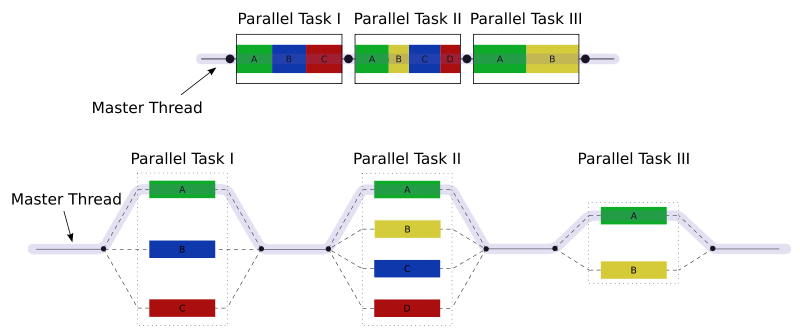
\includegraphics[width=1.0\textwidth]{forkjoin.png}
\caption{Modelo paralelo \textit{Fork-Join} usado por \textit{OpenMP}.\label{fig:forkjoin}}
\end{figure}

Otro API de programaci�n utilizado para plataformas de memoria compartida basadas en GPU es \textit{CUDA}\cite{progparmachines}. Las GPUs son m�quinas SIMD seg�n la taxonom�a de Flynn (v�ase Secci�n \ref{sec:flynn}) utilizando el modelo de memoria compartida. Una diferencia con los multicores que tambi�n utilizan este modelo, es que las GPUs pueden tener miles de hilos corriendo simult�neamente. Un programa en CUDA tiene dos partes, el c�digo que se ejecuta en el \textit{host} o procesador central (CPU), y el c�digo que se ejecuta en el \textit{device} (GPU) llamado \textit{kernel}. Debido a esto es necesaria una CPU que trabaje en conjunto con la GPU. Cualquier aplicaci�n que siga encaje en el modelo SIMD, donde se apliquen las mismas instrucciones a un conjunto de datos, se ver� muy beneficiada en el uso de una GPU. Cualquier otro tipo de aplicaci�n no es factible en estas plataformas.\\

\subsection{Paso de mensajes}

En este modelo, la plataforma consiste en una serie de nodos de procesamiento interconectados, cada uno con su propio espacio de direcciones de memoria. Cada nodo puede ser un solo procesador, o un multiprocesador con espacio de memoria compartido entre sus cores. En este modelo, la interacci�n entre procesos corriendo en distintos nodos se realiza mediante en el env�o de mensajes.\\

Los mensajes proporcionan un modo de transferir datos, tareas y sincronizar procesos. Puesto que la interacci�n se consigue mediante envio/recepci�n de mensajes, las operaciones b�sicas de este paradigma de programaci�n son \textit{send} y \textit{receive}. Es necesario adem�s un mecanismo que asigne un ID �nico a cada proceso que permita identificarlo en un programa paralelo con m�ltiples procesos, puesto que los mensajes necesitan un ID de destino para ser entregados. Un proceso podr�a saber pues su ID introduciendo la operaci�n \textit{whoami}.\\

Otra funci�n necesaria es \textit{numprocs} que diga al proceso el n�mero de procesos que intervienen en el programa paralelo. Con las cuatro operaciones introducidas anteriormente se puede implementar cualquier programa de paso de mensajes. Algunas de las implementaciones de paso de mensaje m�s utilizadas son Message Passing Interface (MPI) y Parallel Virtual Machine (PVM).\\ 

\textit{Message Passing Interface}\cite{progparmachines,openmpquinn,usingmpi} es un est�ndar de facto para el modelo de programaci�n paralela mediante paso de mensajes. MPI, al igual que OpenMP, es una API usada generalmente en entornos C/C++ entre otros. Tiene implementaciones tanto en c�digo libre, como propietarias. Entre las implementaciones m�s conocidas se encuentran \textit{Open MPI}, \textit{LAM} y \textit{MPICH}.\\

La forma de procesar, en un entorno MPI, un programa consiste en ejecutar copias de ese programa (procesos) en tantas m�quinas como se quieran utilizar. Cada copia se encarga de procesar una parte de los datos de entrada intercambiando informaci�n, mediante paso de mensajes, por la red.MPI permite distintas clases de comunicaci�n en los sistemas que la utilizan. En las comunicaciones colectivas interviene un nodo que interact�a con los dem�s, ya sea que todos le manden informaci�n al mismo o que este env�e informaci�n a todos. Tambi�n permite las comunicaciones punto a punto. Adem�s, estas dos clases de comunicaci�n tienen dos variantes: bloqueantes y no bloqueantes.\\

Adicionalmente, existe una API basada en MPI para operaciones I/O en sistemas paralelos de almacenamiento, se llama \textit{MPI-IO}\cite{usingmpi}. Esta API es la parte de MPI que maneja el I/O, ofreciendo distintas operaciones de lectura y escritura. Permite adem�s determinar como se van a distribuir los datos entre los procesos, y como se van a almacenar los datos en disco una vez procesados. Esto permite solucionar las limitaciones de memoria al procesar ficheros muy grandes (no hay que cargarlos en la memoria de una sola m�quina) y obtener un �nico fichero de salida.\\

\subsection{Partitioned Global Address Space - PGAS}

El modelo de PGAS\cite{intropgas} se caracteriza por ofrecer al programador un espacio de memoria �nico y compartido en un sistema con memoria distribuida. Mediante una capa interfaz, se ofrece a los nodos (que tiene cada uno su memoria local) una forma de utilizar tambi�n las memorias locales de los otros nodos del sistema. Lo que esto ofrece al programador es una visi�n local de todo el espacio de memoria como uno �nico y global, transparencia en las comunicaciones (puesto que el compilador se encarga de las mismas) y soporte para datos distribuidos.\\

A nivel de nodo, la variables de memoria pueden ser \textit{shared} o \textit{local}, permitiendo compartir �nicamente las variables que interesan para la comunicaci�n y no sobrecargando la comunicaci�n con variables auxiliares y privadas que solo le sirven al nodo local. Algunos APIs de programaci�n que utilizan este modelo son \textit{Unified Parallel C}, \textit{Co-Array Fortran}, \textit{Titanium}, \textit{X-10} y \textit{Chapel}.\\

\subsection{OmpSS}

OmpSS\cite{gpuompss} es un modelo de programaci�n que utiliza como base OpenMP, modific�ndolo para soportar paralelismo irregular, as�ncrono y en plataformas heterog�neas. Utiliza un modelo de \textit{pool} de hilos en lugar de \textit{fork-join}(usado por OpenMP), donde un hilo maestro crea los trabajos y el resto de hilos los procesan. Otra diferencia es la distinci�n de varios espacios de memoria de cada nodo, al contrario del �nico espacio de memoria de OpenMP. Es el propio compilador el que se encarga de distribuir los datos y elegir en qu� dispositivo procesarlos.\\
%\subsection{APIs de programaci�n paralela}
En este apartado se presentar�n algunas de las interfaces de programaci�n (API) m�s utilizas en la elaboraci�n de programas paralelos. Estas API se pueden ajustar siempre a uno de los dos modelos de memoria que ya se han visto: memoria compartida y memoria distribuida (o paso de mensajes). Se comentar� brevemente el modo de funcionamiento de estas API y algunas de sus caracter�sticas.\\

\subsubsection{POSIX threads}
Los POSIX\cite{advunix} (\textit{Portable Operating System Interface uniX}) threads (a partir de ahora \textit{pthreads}) se basan en el concepto de hilo o thread, que la mayor�a de sistemas operativos actuales utilizan.\\

En un sistema UNIX, un proceso no es mas que un �nico hilo de control. Este hilo podr�a replicarse para crear m�s hilos ``hijos'', permitiendo que cada uno de estos hilos se dedique a ejecutar una tarea distinta a los dem�s. Esto permite no solo ejecutar un programa con varios hilos ejecut�ndose en paralelo, sino que permite abstraer el programa en ta\-reas definidas, independientemente del n�mero de procesadores que tengamos. Estos hilos tambi�n comparten memoria, por lo que se utiliza un modelo de memoria compartida.\\

Pthreads\cite{advunix} es la interfaz de programaci�n con hilos que ofrecen las librer�as POSIX. Esta interfaz nos ofrece funciones simples y potentes necesarias para crear cualquier c�digo que utilice hilos.\\

Programar con hilos nos ofrece algunas ventajas. Podemos simplificar el c�digo para manejar eventos as�ncronos, simplemente destinando un thread a manejar cada uno de esos eventos de forma s�ncrona. Adem�s, es m�s f�cil comunicarse entre hilos del mismo proceso que entre procesos distintos, puesto que los hilos comparten el mismo espacio de memoria y los descriptores de ficheros. Tambi�n es posible mejorar el rendimiento en programas interactivos, asignando hilos a procesar la respuesta del usuario y otros hilos al resto de tareas.\\

Por �ltimo comentar que en un sistema multiprocesador, un programa con hilos se ejecutar� (probablemente) m�s r�pido que en uno uniprocesador, pero a�n as�, en un sistema uniprocesador el proceso podr�a ejecutarse tambi�n m�s r�pido si utiliza hilos. Esto podr�a deberse a que mientras unos hilos est�n bloqueados (esperando el resultado de operaciones I/O por ejemplo), otros hilos pueden continuar su ejecuci�n.\\

\subsubsection{OpenMP}
\textit{OpenMP}\cite{openmpquinn,openmpchandra,openmpreview} es un API de programaci�n paralela (basada en directivas del compilador, rutinas de librer�a y variables de entorno), en C/C++ y Fortran, para multiprocesadores de memoria compartida. Puede correr en sistemas Unix y Windows NT. Sus caracter�sticas m�s importantes residen en su simplicidad y flexibilidad, ofreciendo una interfaz que permite crear programas paralelos tanto para sistemas sobremesa como supercomputadores.\\

OpenMP utiliza por debajo el modelo fork-join (Figura \ref{fig:forkjoin}) para llevar a cabo las tareas paralelas. Adem�s se asegura una ejecuci�n correcta tanto en sistemas paralelos como secuenciales (siempre y cuando sea correctamente utilizado).\\

\begin{figure}
\centering
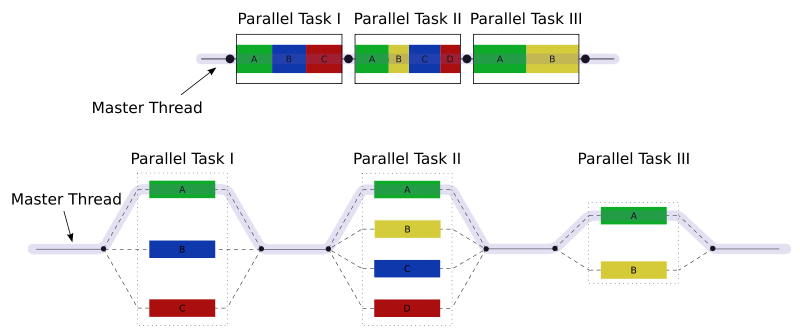
\includegraphics[width=1.0\textwidth]{forkjoin.png}
\caption{Modelo paralelo \textit{Fork-Join} usado por \textit{OpenMP}.\label{fig:forkjoin}}
\end{figure}

Como cualquier proceso Unix, un programa que utiliza OpenMP comienza con un �nico hilo inicial que se ejecuta secuencialmente y que da lugar a m�s hilos. Otra caracter�stica de OpenMP es que no garantiza que las operaciones I/O se realicen de forma s�ncrona cuando se hace de forma paralela, para ello ofrece mecanismos de sincronizaci�n que la propia API ofrece.\\

OpenMP utiliza el modelo de memoria compartida para ejecutar sus hilos. Permite que los hilos compartan espacio de memoria, pero tambi�n permite que tengan su propio espacio de memoria privada. Adem�s permite a los hilos tener un snapshot de la memoria en cualquier momento, y utilizar esa informaci�n mientras el resto de hilos pueden seguir modificando la memoria sin afectar al snapshot.\\

La API soporta el paralelismo a nivel de bucle, paralelismo anidado (hilos hijos pueden crear a su vez nuevos hilos hijos de estos) y paralelismo por tareas (cada hilo se encarga de un trozo de c�digo).\\

\subsubsection{MPI}
\textit{Message Passing Interface}\cite{progparmachines,openmpquinn,usingmpi} es un estandard de facto para el modelo de programaci�n paralela mediante paso de mensajes. MPI surgi� como necesidad para permitir la programaci�n paralela en el auge de los \textit{NOWs}. Un sistema de memoria compartida era entonces caro, por lo que se buscaba una alternativa viable.\\

MPI, al igual que OpenMP, es una API usada generalmente en entornos C/C++ entre otros. Tiene implementaciones tanto en c�digo libre, como propietarias. Entre las implementaciones m�s conocidas se encuentran \textit{Open MPI}, \textit{LAM} y \textit{MPICH}.\\

La forma de procesar, en un entorno MPI, un programa consiste en ejecutar copias de ese programa (procesos) en tantas m�quinas como se quieran utilizar. Cada copia se encarga de procesar una parte de los datos de entrada intercambiando informaci�n, mediante paso de mensajes, por la red.\\

Dependiendo de la red, MPI puede introducir una sobrecarga importante si la comunicaci�n entre procesos es fluida. Por ejemplo en sistemas cluster los procesos en distintos nodos comunicados mediante una red t�pica \textit{Infiniband} har�n el trabajo generalmente m�s r�pido cuanta menos comunicaci�n haya entre ellos. En cambio en un sistema de memoria compartida como un multiprocesador o un multicore, la red es mucho m�s r�pida por lo que la sobrecarga es menor. Incluso algunas implementaciones, podr�an aprovechar la memoria compartida de estos sistemas para optimizar la comunicaci�n.\\

MPI permite distintas clases de comunicaci�n en los sistemas que la utilizan. En las comunicaciones colectivas interviene un nodo que interact�a con los dem�s, ya sea que todos le manden informaci�n al mismo o que este env�e informaci�n a todos. Tambi�n permite las comunicaciones punto a punto. Adem�s, estas dos clases de comunicaci�n tienen dos variantes: bloqueantes y no bloqueantes.\\

Existe una API basada en MPI para operaciones I/O en sistemas paralelos de almacenamiento, se llama \textit{MPI-IO}\cite{usingmpi}. Esta API es la parte de MPI que maneja el I/O, ofreciendo distintas operaciones de lectura y escritura. Permite adem�s determinar como se van a distribuir los datos entre los procesos, y como se van a almacenar los datos en disco una vez procesados. Esto permite solucionar las limitaciones de memoria al procesar ficheros muy grandes (no hay que cargarlos en la memoria de una sola m�quina) y obtener un �nico fichero de salida.\\

\subsubsection{CUDA}

Debido a la industria del videojuego, las GPUs han evolucionado enormemente en estos �ltimos a�os, permitiendo procesar im�genes cada vez m�s r�pido.y m�s reales. Esta evoluci�n hizo plantearse si se podr�an usar para algo m�s que no fuesen s�lo gr�ficos.\\

Todo esto desemboca con \textit{NVIDIA} desarrollando un lenguaje de programaci�n para sus GPUs, denominado \textit{CUDA}\cite{progparmachines}. Las GPUs son m�quinas SIMD seg�n la taxonom�a de Flynn (v�ase Secci�n \ref{sec:flynn}) y utilizan el modelo de memoria compartida. Una diferencia con los multicores que tambi�n utilizan este modelo, es que las GPUs pueden tener miles de hilos corriendo simult�neamente.\\

Un programa en CUDA tiene dos partes, el c�digo que se ejecuta en el \textit{host} o procesador central (CPU), y el c�digo que se ejecuta en el \textit{device} (GPU) llamado \textit{kernel}. Debido a esto es necesaria una CPU que trabaje en conjunto con la GPU.\\

Cualquier aplicaci�n que siga encaje en el modelo SIMD, donde se apliquen las mismas instrucciones a un conjunto de datos, se ver� muy beneficiada en el uso de una GPU. Cualquier otro tipo de aplicaci�n no es factible en estas plataformas.\\

\subsubsection{OpenCL}

OpenCL\cite{openclprog} es un API de programaci�n para sistemas compuestos por CPUs, GPUs y otros tipos de procesadores (sistemas heterog�neos). OpenCL te permite escribir programas que puedan corren en un amplio conjunto de sistemas, desde celulares hasta nodos de un cluster.\\

A diferencia de otros APIs, OpenCL expone el hardware e informa de sus caracter�sticas al programador. As�, el programador decide como distribuye los datos entre los dispositivos que tiene disponibles. Tambi�n ofrece un modelo de programaci�n de alto nivel que abstrae las caracter�sticas hardware.\\

OpenCL permite descubrir que componentes forman el sistema. Adem�s testea esos componentes para determinar sus caracter�sticas, as� el software puede adaptarse. Similar al procesamiento en GPUs, la API crea bloques de instrucciones (kernels) que se ejecutar�n en el sistema en un determinado orden y en determinados dispositivos.\\
\section{Tratamiento de grandes cantidades de datos}

Una de las caracter�sticas m�s significativas en el tratamiento de genoma, es la gran cantidad de datasets que se generan. Estos datos hay que manejarlos de forma eficiente y adecuada, para preservar su integridad y a la vez que su acceso sea lo m�s r�pido posible. Esta secci�n est� dedicada a distintos modelos que se utilizan hoy d�a para el tratamiento de una gran cantidad de datos.

\subsection{MapReduce}

MapReduce\cite{mapreducesimp} es un modelo de programaci�n con una implementaci�n asociada para procesar y generar grandes datasets. En los �ltimos a�os se han venido implementando cientos de c�digos de prop�sito especial (Google implement� la mayor�a) para procesar grandes cantidades de datos en bruto, c�mo documentos o peticiones web, para obtener distintos tipos de informaci�n derivada (�ndices, grafos de webs, res�menes...). La mayor�a de estos procesos son triviales y no requieren de un computo intensivo, pero los datos de entrada son demasiado grandes y tienen que ser distribuidos entre miles de m�quinas para procesarlos en un tiempo razonable.\\

Todo esto generaba cada vez m�s complejidad, por lo que la reacci�n fue el dise�o de un nuevo tipo de abstracci�n que permitiese realizar simples c�mputos ocultando detalles del paralelismo, la distribuci�n de los datos y la carga, ofreciendo adem�s tolerancia a fallos. Todo esto incluido en una simple librer�a, as� fue como naci� MapReduce (de mano de Google).\\

El computo en este modelo se basa en un conjunto de pares clave/valor de entrada, que generan un conjunto de pares clave/valor de salida. Esto se genera mediante dos funciones que el programador debe definir: \textit{Map} y \textit{Reduce}. \textit{Map} obtiene un par de entrada y genera un conjunto de pares intermedios. Estos pares intermedios son recopilados internamente por la librer�a y los agrupa por su clave intermedia, pas�ndolos seguidamente a la funci�n \textit{Reduce}. La funci�n \textit{Reduce} acepta una de las claves intermedias y el conjunto de valores para esa clave, combin�ndolos para generar el conjunto de valores de salida. La Figura \ref{fig:mapreduce} muestra gr�ficamente un ejemplo para contar palabras usando el modelo \textit{MapReduce}.\\


\begin{figure}
\centering
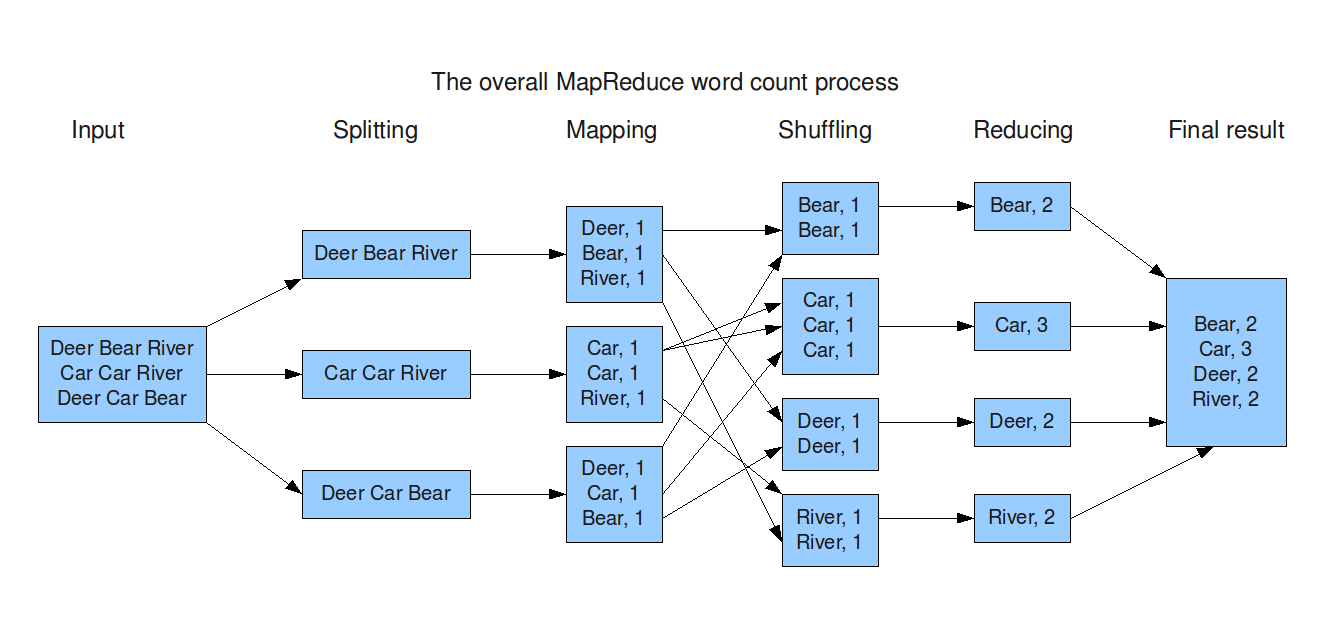
\includegraphics[width=0.8\textwidth]{mapreduce.png}
\caption{Modelo paralelo \textit{MapReduce} para contar palabras.\label{fig:mapreduce}}
\end{figure}
\chapter{Estado del Arte: Bioinform�tica}

En los �ltimos a�os se han producido avances en las tecnolog�as de secuenciaci�n que han aumentado la productividad a una escala sin precedentes, con lo que la bioinform�tica ha encontrado dificultades para almacenar y analizar esas grandes cantidades de datos. Se habla de que la biolog�a ha entrado en la era del \textit{``big data''}, enfrent�ndose a nuevos retos como son el almacenamiento, an�lisis, b�squeda, difusi�n y visualizaci�n de los datos que requieren nuevas soluciones.\\

En esta secci�n se ver�n algunas de las herramientas y lenguajes de programaci�n m�s utilizados para abordar los problemas de an�lisis gen�mico y cuales son sus caracter�sticas m�s relevantes. Se�alar que no son las �nicas y que existen m�s, tanto de prop�sito especifico (la mayor�a) como general.\\

\section{Bioconductor}

\textit{Bioconductor} \cite{bioconductor} es un software open-source, de libre desarrollo que proporciona herramientas para el an�lisis y comprensi�n de los datos de gen�mica. Est� basado en el lenguaje de programaci�n \textit{R}\cite{rproject}. Las herramientas que proporciona est�n contenidas en paquetes de \textit{R} por lo que es orientado a objetos y le proporciona ciertas caracter�sticas: un lenguaje interpretado de alto nivel para un r�pido prototipado de nuevos algoritmos, sistema de paquetes, acceso a datos de gen�mica online, soporte completo estad�stico y capacidades de visualizaci�n de los modelos.\\

Los paquetes est�n bien documentados, incluso con ejemplos de uso. Ofrece adem�s las herramientas junto con un flujo de trabajo a seguir para realizar distintos an�lisis y mostrar sus resultados de forma gr�fica.\\

\section{Bioperl}

\textit{Bioperl} \cite{bioperl} es un conjunto de herramientas bioinform�ticas basadas en m�dulos del lenguaje de programaci�n \textit{Perl}. Est� orientado a objetos, por lo que para llevar a cabo una tarea, algunos m�dulos necesitar�n de otros para llevar a cabo su funci�n. Posee, entre otras cosas, interfaces gr�ficas, almacenamiento persistente en bases de datos y procesadores de los resultados de varias de aplicaciones para poder usarlos. Se utiliza para producir nuevas herramientas m�s complejas.\\

\section{Genome Analysis ToolKit}

\textit{Genome Analysis Toolkit} \cite{gatkframework, gatkweb} (\textit{GATK}) es el estandard de facto para el an�lisis y descubrimiento de variantes de genoma. Es un conjunto de herramientas gen�rico que pueden ser aplicadas a cualquier tipo de conjunto de datos y problemas de an�lisis de genoma, ya que se puede usar tanto para descubrimiento como para validaci�n.\\

Soporta datos provenientes de una amplia variedad de tecnolog�as de secuenciaci�n y aunque inicialmente se desarroll� para gen�tica humana, actualmente puede manejar el genoma de cualquier organismo. \textit{GATK} ofrece una estructura o \textit{framework} que se ocupa de ejecutar las distintas herramientas sobre los datos de entrada. Estas herra-mientas pueden ser las que trae por defecto el propio programa u otras desarrolladas por los usuarios, permitiendo cualquier combinaci�n compatible de las mismas. \textit{GATK} sugiere varios flujos de trabajo a seguir para conseguir determinados resultados, pero se pueden realizar otros flujos personalizados.\\

Los requerimientos del programa son �nicamente un sistema compatible con \textit{POSIX} y Java instalado. Ofrece tambi�n la posibilidad de mostrar los resultados gr�ficamente usando \textit{R}. En cuanto al rendimiento, utiliza un sistema \textit{MapReduce} para particionar el trabajo a realizar sobre la gran cantidad de datos de entrada y utiliza hilos para acelerar el proceso.\\

Para el procesamiento a gran escala utiliza una estrategia que consiste en partir los datos de entrada y ejecutar cada parte en distintas m�quinas independientemente, llamada \textit{scatter-gather}. En la Figura \ref{fig:gatkqueue} se representa el modelo \textit{scatter-gather} que utiliza \textit{GATK} donde cada tarea naranja ser�a una instancia distinta del programa.\\

\begin{figure}
\centering
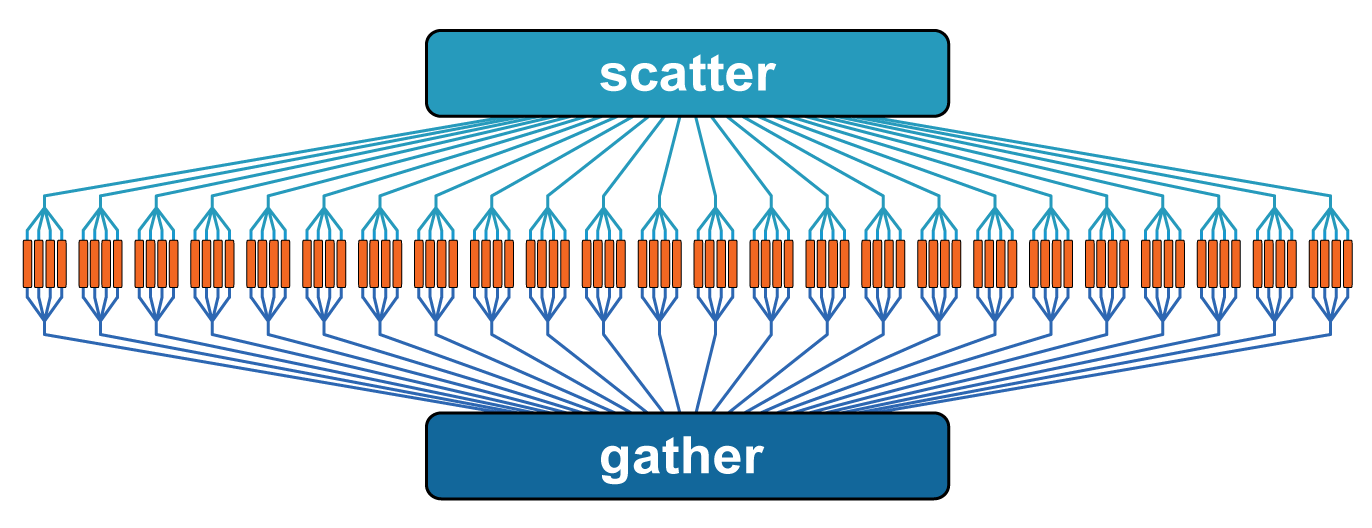
\includegraphics[width=0.8\textwidth]{queuegatk.png}
\caption{Modelo paralelo utilizado por \textit{GATK} para el procesamiento en \textit{cluster}.\label{fig:gatkqueue}}
\end{figure}

En el aspecto del rendimiento, se echa en falta un procesamiento paralelo a nivel de \textit{cluster} que permita a una tarea terminar antes y no tanto hacer varias a la vez. Adem�s, no se centra en obtener un alto rendimiento, en parte por usar Java, prefiriendo la facilidad de programaci�n y la portabilidad que ofrece este lenguaje de programaci�n.\\

\section{Bowtie}

\textit{Bowtie} \cite{bowtieweb} es un alineador de lecturas cortas de genoma (prop�sito espec�fico) muy r�pido y eficiente con la memoria. Este programa es muy usado pero tiene el inconveniente de que solo sirve para el alineamiento. Se puede utilizar como herramienta de altas prestaciones al inicio de un flujo de trabajo que utilice otras herramientas que la complementen. Este programa puede utilizar los \textit{cores} del procesador usando hilos pero no tiene soporte interno al procesamiento en \textit{cluster}.\\

\section{OpenCB}

\textit{OpenCB} \cite{opencb} es un proyecto que nace como alternativa a los proyectos que normalmente se focalizan en un lenguaje de programaci�n como el de Bioconductor o Bioperl. Este grupo proporciona software avanzado y open-source para el an�lisis de datos de gen�mica con una alta productividad.\\

El proyecto est� organizado en cuatro subproyectos diferentes, cada uno centrado en resolver un problema concreto. Estos son el \textit{``High-Performance Genomics''} (HPG), centrado en acelerar los an�lisis usando tecnolog�as \textit{HPC} (High Performance Computing); \textit{``Cloud computing''}, para almacenar y difundir los datos; \textit{``Distributed NoSQL databases''}, para manejar la gran cantidad de datos; y \textit{``Big data visualization''}, para obtener una representaci�n visual de los resultados.\\

\textit{HPG} es un proyecto escalable, de alto rendimiento y open-source, que consiste en diferentes herramientas y algoritmos para el an�lisis de datos a escala gen�mica. Utiliza HPC para acelerar los algoritmos y las herramientas para el an�lisis, usando el lenguaje de programaci�n C y buscando los algoritmos que mejor se ajustan a cada problema en concreto. Se busca tambi�n la escalabilidad, que permita acelerar las ejecuciones cuantos m�s recursos computacionales est�n disponibles.\\

\section{Conclusiones}

En esta \textit{tesis} tenemos como referencia la \textit{suite} de herramientas del \textit{GATK} puesto que es la m�s utilizada. La raz�n de la elecci�n radica en que aun siendo la m�s utilizada, no es una herramienta pensada para ofrecer un alto rendimiento. A pesar de esto, sus ventajas son la facilidad a la hora de procesar cualquier \textit{dataset} de entrada, sea cual sea el secuenciador que lo haya generado. Esto unido a la capacidad para procesar el \textit{dataset}, sea del tama�o que sea, y la posibilidad de aplicarle cualquier algoritmo justifican el amplio uso de esta herramienta.\\

En cuanto a sus desventajas, la principal es la falta de rendimiento como ya se ha comentado. La herramienta en s� hace su trabajo y obtiene resultados, pero no es factible para una aplicaci�n cotidiana, por ejemplo, al �mbito de la sanidad (donde no es lo mismo que se obtengan los resultados de un paciente a los 2 meses que a las 2 horas).\\

Lo que se pretende por tanto es replicar esta herramienta para conservar sus ventajas pero intentando eliminar sus desventajas. Para ello se aplicar�n t�cnicas de computaci�n de altas prestaciones, usando lenguajes de programaci�n eficientes con memoria y los recursos del sistema y adem�s llevando la ejecuci�n al �mbito de los sistemas multiprocesador.\\
%\chapter{Estado del arte: �Conclusiones?�Factores a tener en cuenta?�Lo meto en el capitulo de trabajo de investigaci�n?}

\section{Modelo de programaci�n paralela a tener en cuenta}

Es interesante la aplicaci�n de ambos modelos de programaci�n en la elaboraci�n de esta \textit{tesis}, a distintos niveles. Podemos utilizar el modelo de memoria compartida a nivel de procesador, puesto que hoy d�a los nuevos procesadores son mayoritariamente un sistema \textit{SMP} \textit{on-chip} con varios n�cleos de procesamiento y que comparten la misma memoria principal. Podemos usar este modelo de programaci�n para acelerar los tiempos de ejecuci�n dentro del procesador, usando con la m�xima eficiencia posible todos los n�cleos de procesamiento del mismo.\\

Podemos aplicar igualmente el modelo de paso de mensajes para llevar la ejecuci�n a un entorno multiprocesador o un \textit{cluster}. Mediante este modelo podemos acelerar el tiempo de ejecuci�n de los programas usando en paralelo los procesadores de los que se dispone en un sistema tipo \textit{cluster}. Con ello se busca mayor velocidad de computo cuantos m�s recursos (procesadores) disponga el sistema.\\

El modelo de \textit{PGAS} en cambio no se considera factible su uso en esta \textit{tesis}. Esto es debido a que la capa de virtualizaci�n, para dar la visi�n de memoria compartida, es costosa tanto econ�micamente como en prestaciones. Debido a la sobrecarga a la que somete al sistema y puesto que estamos en entornos de altas prestaciones, no se utilizar� al no considerarse necesaria.\\

Podemos concluir por tanto en el uso del modelo de memoria compartida combinado con el modelo de paso de mensajes, cada uno acelerando el tiempo de ejecuci�n a distintos niveles en un sistema multiprocesador.\\

\section{Tratamiento de datos}

\section{Software referencia de bioinform�tica para esta tesis}

En esta \textit{tesis} tenemos como referencia la \textit{suite} de herramientas del \textit{GATK} puesto que es la m�s utilizada. La raz�n de la elecci�n radica en que aun siendo la m�s utilizada, no es una herramienta pensada para ofrecer un alto rendimiento. A pesar de esto, sus ventajas son la facilidad a la hora de procesar cualquier \textit{dataset} de entrada, sea cual sea el secuenciador que lo haya generado. Esto unido a la capacidad para procesar el \textit{dataset}, sea del tama�o que sea, y la posibilidad de aplicarle cualquier algoritmo justifican el amplio uso de esta herramienta.\\

En cuanto a sus desventajas, la principal es la falta de rendimiento como ya se ha comentado. La herramienta en s� hace su trabajo y obtiene resultados, pero no es factible para una aplicaci�n cotidiana aplicada, por ejemplo, al �mbito de la sanidad (donde no es lo mismo que se obtengan los resultados de un paciente a los 2 meses que a las 2 horas).\\

Lo que se pretende por tanto es replicar esta herramienta para conservar sus ventajas pero intentando eliminar sus desventajas. Para ello se aplicar�n t�cnicas de computaci�n de altas prestaciones, usando lenguajes de programaci�n eficientes con memoria y los recursos del sistema y adem�s llevando la ejecuci�n al �mbito de los sistemas multiprocesador.\\
\chapter{Anteproyecto de Tesis}

Primeramente se describir� en qu� consiste el proceso de descubrimiento de variantes, dando una breve introducci�n a la gen�tica y al \textit{ADN}. Se describir� desde d�nde se parte y cuales son los objetivos a cumplir durante la realizaci�n de esta tesis. Finalmente se presentar� un desglose de las tareas que se llevar�n a cabo para alcanzar los objetivos propuestos y cu�l ser� su planificaci�n.\\

\section{Introducci�n al descubrimiento de variantes}

\subsection{ADN}

El \textit{ADN} \cite{molecularbio} (�cido desoxirribonucleico) contiene las instrucciones gen�ticas usadas en el desarrollo y funcionamiento de todos los organismos vivos conocidos y algunos virus, y es responsable de su transmisi�n hereditaria. Se puede comparar el ADN con una receta o c�digo, ya que a partir del mismo se obtienen las instrucciones necesarias para construir las c�lulas. Los segmentos de ADN que contienen esta informaci�n son los denominados genes, mientras que el resto de secuencias tienen prop�sitos estructurales y reguladores en el uso de esta informaci�n. En la Figura \ref{fig:adn} tenemos la representaci�n gr�fica que muestra d�nde reside el ADN.\\

\begin{figure}
\centering
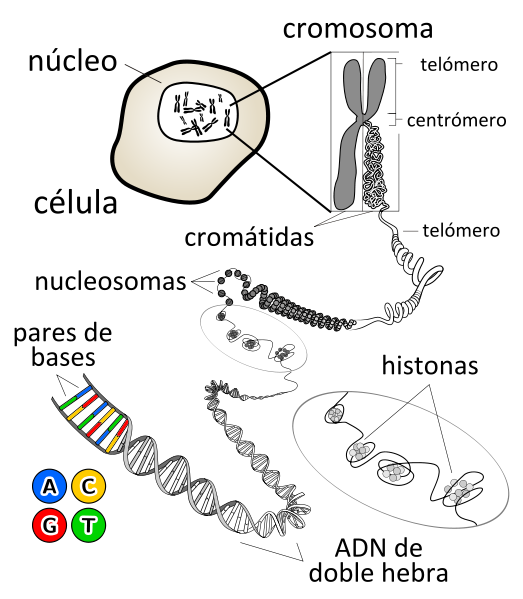
\includegraphics[width=0.5\textwidth]{adn.png}
\caption{�D�nde se encuentra el ADN? \cite{adnwiki}.\label{fig:adn}}
\end{figure} 

El ADN es un pol�mero de nucle�tidos formado por muchas unidades simples (nucle�tidos) conectadas entre s� (Figura \ref{fig:adnquimic}). Los nucle�tidos est�n formados por un az�car, una base nitrogenada (pueden ser Adenina, Timina, Citosina y Guanina) y un grupo fosfato para interconectarlos. Puesto que lo �nico que distingue a un nucle�tido de otro es la base nitrogenada, la secuencia de ADN se representa por una secuencia de estas bases. En estas secuencias cada base se representa por su inicial, por lo que tienen una representaci�n del tipo \textit{AGTCTAGATCG}\ldots En los organismos vivos el ADN se presenta como una doble cadena de nucle�tidos.\\

\begin{figure}
\centering
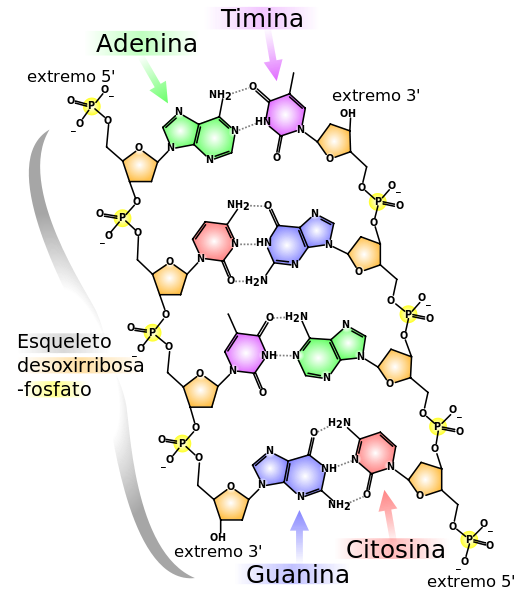
\includegraphics[width=0.4\textwidth]{adnquimic.png}
\caption{Representaci�n qu�mica del ADN \cite{adnwiki}.\label{fig:adnquimic}}
\end{figure} 

Como ya se ha dicho, un gen es una secuencia del ADN que contiene informaci�n gen�tica, concretamente es una unidad de herencia que influye en una caracter�stica particular de un organismo (como el color de los ojos, por ejemplo). A partir de los genes se producen las prote�nas del organismo, que son las encargadas de generar los m�sculos, pelo, enzimas\ldots\\

\subsection{Descripci�n del proceso de descu\-bri\-mien\-to de variantes}

Puesto que un cambio en el ADN puede traducirse en un cambio brusco de las prote�nas que genera el organismo, esto puede dar lugar a trastornos, enfermedades, etc. El proceso de descubrimiento de variantes tiene como objetivo localizar variaciones, mutaciones o \textit{indels} (\textit{insertions/deletions}) en una muestra de ADN con respecto a otra, por ejemplo para poder determinar la causa de enfermedades o prevenirlas.\\

Un ejemplo ser�a analizar el ADN de una poblaci�n (conjunto de individuos) que tengan un determinado tipo de c�ncer y otra poblaci�n que no lo tengan. Estos individuos tendr�n muchas similitudes en el ADN puesto que pertenecen a la misma especie, pero tambi�n diferir�n en otras. Cuando encontremos la secuencia de ADN com�n a la poblaci�n con c�ncer, pero que no aparezca en la poblaci�n sin c�ncer, tendremos la raz�n de ese c�ncer localizada y podremos tratarlo y prevenirlo.\\

El proceso de descubrimiento de variantes tiene tres fases. En la primera fase se obtienen lecturas de ADN en un formato espec�fico y dependiente de la plataforma que las haya obtenido. Lo que se hace con estas lecturas es transformarlas a un �nico formato gen�rico, con unas calidades bien calibradas, mapeadas y alineadas con su ADN de referencia. El formato utilizado es el \textit{SAM/BAM} \cite{bamsam} (\textit{Sequence Aligment Map/Binary Alignment Map}), el cual es independiente de la tecnolog�a de obtenci�n del ADN.\\

En la segunda fase se analizan los ficheros \textit{SAM/BAM} para obtener posiciones del ADN que, seg�n evidencia estad�stica, sean mutaciones respecto al ADN de referencia. Esto incluye diferencias en una sola posici�n de la cadena de ADN (\textit{SNP}, \textit{Single Nucleotide Polymorphism}), peque�os \textit{indels}, etc. Esta fase genera ficheros \textit{VCF} (\textit{Variant Call Format}) que contienen las diferencias con el ADN referencia.\\

En la �ltima fase se analizan las mutaciones obtenidas y la estructura del ADN para generar conclusiones. En la Figura \ref{fig:procesodescubrimiento} se puede ver gr�ficamente estas tres fases.\\

\begin{figure}
\centering
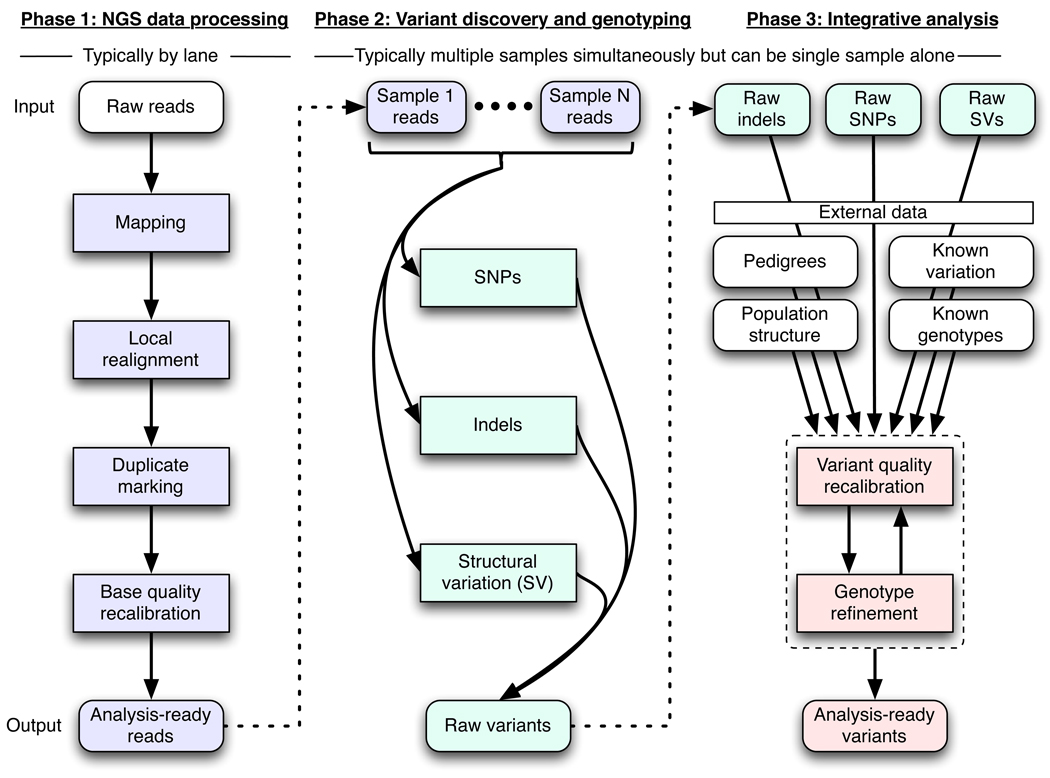
\includegraphics[width=0.8\textwidth]{variationdiscover.jpg}
\caption{Proceso de descubrimiento de variantes en el ADN \cite{gatkframework}.\label{fig:procesodescubrimiento}}
\end{figure} 

\section{Punto de partida}

GATK ser� la herramienta de referencia para la realizaci�n de esta tesis, abarcando parte de la primera fase y la segunda del proceso de descubrimiento de variantes. Seg�n la Figura \ref{fig:procesodescubrimiento}, se quiere implementar el recalibrado de las calidades de las bases (\textit{Base quality recalibration}) de la primera fase del descubrimiento de variantes, desarrollando un recalibrador. Tambi�n se quiere implementar la segunda fase completa, desarrollando un descubridor de variantes.\\

Las implementaciones tendr�n que ser eficientes y aprovechar al m�ximo todos los recursos computacionales de los que se disponga en el entorno que se ejecuta, por ejemplo en un \textit{cluster}. GATK no incorpora completamente estas caracter�sticas, puesto que solo aprovecha la capacidad de proceso mediante hilos y no utiliza estructuras de datos eficientes ni gesti�n de memoria �ptima (en parte por utilizar Java).\\

\section{Objetivos}

\subsection{Objetivo general}

Desarrollar herramientas que permitan realizar el recalibrado de las calidades de las bases (\textit{Base quality recalibration}) y toda la segunda fase del descubrimiento de variantes. Estas herramientas deber�n ser eficientes con los recursos computacionales y con la gesti�n de memoria.\\

\subsection{Objetivos espec�ficos}

El objetivo general de la tesis se puede desglosar en una serie de objetivos espec�ficos, que mediante su cumplimiento permitir�n alcanzar el objetivo general:

\begin{itemize}
\item
Implementar un recalibrador que realice el recalibrado de la calidad de las bases y genere ficheros BAM ya recalibrados.
\item
Implementar un descubridor de variantes que realice toda la segunda fase de descubrimiento de variantes y genere ficheros de resultados VCF.
\item
Desarrollar implementaciones lo m�s eficientes posible, utilizando tecnolog�as paralelas que permitan explotar los recursos de c�mputo disponibles en cada situaci�n.
	\begin{itemize}
	\item
	Usar las tecnolog�as disponibles en los microprocesadores para acelerar la ejecuci�n.
	\item
	Usar las capacidades de memoria compartida de los procesadores \textit{multicore}.
	\item
	Usar las capacidades de paso de mensaje de los sistemas multiprocesador o \textit{clusters}.
	\item
	Mantener las comunicaciones entre procesos al m�nimo.
	\item
	Reducir el n�mero de operaciones I/O al m�nimo. 
	\end{itemize}
\item
Usar estructuras de datos �ptimas que permitan aprovechar las caracter�sticas de las arquitecturas y el sistema de memoria de los computadores. Explotar la localidad temporal y espacial de los datos en memoria.
\end{itemize}

\section{Planificaci�n de tareas}

En esta secci�n se presenta un listado de las diferentes tareas a llevar a cabo para la consecuci�n de los objetivos anteriormente marcados en este cap�tulo. En la Figura \ref{fig:gantt} se muestra la planificaci�n temporal de estas tareas mediante un diagrama de Gantt. La tesis doctoral se llevar� a cabo en 4 a�os, habiendo pasado ya casi un a�o en el momento de escribir este documento.\\

La Tabla \ref{tab:tareas} muestra de forma resumida qu� tareas se van a llevar a cabo y su duraci�n aproximada. Hay que destacar que algunas tareas se tienen que realizar durante los 4 a�os de tesis de forma continua, como es la documentaci�n de la propia Tesis y la publicaci�n de resultados o difusi�n. A continuaci�n se describe en detalle en qu� consiste cada una de las tareas.\\

\subsection{Descripci�n de tareas}

En esta secci�n se describir�n las tareas a realizar durante el desarrollo de la tesis doctoral.

\subsubsection{1 - Realizaci�n del m�ster}

Esta tarea consiste en la superaci�n del curso de M�ster de Tecnolog�as Inform�ticas Avanzadas de la Universidad de Castilla-La Mancha. Para ello se superar�n las asignaturas ofertadas por el m�ster que tengan que ver con el tema de investigaci�n. Esta tarea acaba con la realizaci�n de este documento, describiendo el progreso alcanzado durante el primer a�o de tesis, y su defensa ante un tribunal.\\

\subsubsection{2 - Estado del arte}

Esta tarea corresponde a la documentaci�n y estudio del estado del arte en modelos y sistemas de programaci�n paralela, tratamiento de grandes cantidades de datos, y situaci�n actual de las herramientas utilizadas en bioinform�tica para el an�lisis de ADN. Los resultados de este estudio y sus conclusiones se recogen en los cap�tulos de ``Estado del arte'' de este documento.


%\definecolor{LightCyan}   {rgb}{0.88,1.,1.}
%\definecolor{Orange}      {rgb}{1.,0.65,0.}
%\definecolor{PaleGreen}   {rgb}{0.6,0.98,0.6}
%\definecolor{Pink}        {rgb}{1.,0.75,0.8}
%
%\psset{gradmidpoint=0,fillstyle=gradient,gradbegin=LightCyan,gradend=white}
%\newpsstyle{TaskStyleA}{gradbegin=LightCyan,gradend=cyan}
%\newpsstyle{TaskStyleB}{gradbegin=red,gradend=Pink}
%\newpsstyle{TaskStyleC}{gradbegin=yellow,gradend=Orange}
%\newpsstyle{TaskStyleD}{gradbegin=green,gradend=PaleGreen}

\begin{landscape}
\begin{figure}[!htp]
\begin{center}
\makebox[\textwidth]{
\begin{ganttchart}[
	y unit title = 0.3cm,
	y unit chart = 0.4cm,
	vgrid,
	hgrid,
	time slot format=isodate-yearmonth,
	compress calendar,
	today = 2013-06,
	progress = today,
	title/.append style={draw=none, fill=blue!70!white},
	title label font=\sffamily\tiny\bfseries\color{white},
	title left shift=.05,
	title right shift=-.05,
	title height = 1,
	bar/.append style={fill=green!75},
	bar incomplete/.append style={fill=red!75},
	bar label font=\scriptsize\color{black!50},
	group right shift=0,
	group top shift=.3,
	group height=.4,
	group peaks height=.3,
	group label font=\normalsize,
]{2012-07}{2016-07}
\gantttitlecalendar{year,month} \\
%\gantttitlelist{1,...,12}{1} \\
\ganttbar{1-M�ster}{2012-07}{2013-05} \\
\ganttbar{2-Estado arte}{2012-11}{2013-02} \\
\ganttbar{3-Tecnolog�as}{2013-03}{2013-03} \\

%RECALIBRADOR
\ganttgroup{4-Impl. Recalibrador}{2013-03}{2014-03} \\
\ganttbar{4.1-Estructuras datos}{2013-03}{2013-03} \\
\ganttbar{4.2-Implementaci�n}{2013-03}{2013-05} \\
\ganttbar{4.3-Pruebas}{2013-05}{2013-05} \\
%\ganttmilestone{Objetivo 1}{2013-05} \\
\ganttbar{4.4-SSE}{2013-06}{2013-08} \\
\ganttbar{4.5-Pruebas SSE}{2013-08}{2013-08} \\
\ganttbar{4.6-OpenMP}{2013-09}{2013-11} \\
\ganttbar{4.7-Pruebas OpenMP}{2013-11}{2013-11} \\
\ganttbar{4.8-MPI}{2013-12}{2014-03} \\
\ganttbar{4.9-Pruebas MPI}{2014-02}{2014-03} \\
\ganttbar{4.10-Pruebas cluster}{2014-02}{2014-03} \\

%VARIANTES
\ganttgroup{5-Impl. Variantes}{2014-04}{2015-10} \\
\ganttbar{5.1-Estructuras datos}{2014-04}{2014-04} \\
\ganttbar{5.2-Implementaci�n}{2014-04}{2014-07} \\
\ganttbar{5.3-Pruebas}{2014-06}{2014-07} \\
%\ganttmilestone{Objetivo 1}{2013-05} \\
\ganttbar{5.4-SSE}{2014-08}{2014-11} \\
\ganttbar{5.5-Pruebas SSE}{2014-10}{2014-11} \\
\ganttbar{5.6-OpenMP}{2014-12}{2015-03} \\
\ganttbar{5.7-Pruebas OpenMP}{2015-02}{2015-03} \\
\ganttbar{5.8-MPI}{2015-04}{2015-10} \\
\ganttbar{5.9-Pruebas MPI}{2015-06}{2015-10} \\
\ganttbar{5.10-Pruebas cluster}{2015-08}{2015-10} \\

%PUBLICACIONES
\ganttgroup{6-Difusi�n}{2013-10}{2016-04} \\
\ganttbar{6.1-Recalibrador}{2013-10}{2014-11} \\
\ganttbar{6.2-Variantes}{2015-01}{2016-04} \\
\ganttbar{6.3-Doc. tesis}{2014-04}{2016-04} \\

\end{ganttchart}}
\end{center}
\caption{Diagrama Gant: desarrollo de la tesis de doctorado.\label{fig:gantt}}
\end{figure}
\end{landscape}
%%-----------------

\begin{table}
\centering
\resizebox{\textwidth}{!} {
\begin{tabular}{| c | l | p{0.9\textwidth} | c |}
\hline
Num & \textbf{Actividad} 	& \textbf{Descripci�n} & \textbf{Tiempo (meses)}  \\\hline\hline
1 & M�ster 		& Realizaci�n de los cursos del m�ster de tecnolog�as inform�ticas avanzadas & 11 \\\hline
2 &Estado arte & B�squeda de informaci�n y recopilaci�n del estado del arte de las tecnolog�as de computaci�n paralelas y bioinform�tica & 4 \\
3 &Tecnolog�as & Elecci�n de las tecnolog�as a utilizar durante el desarrollo de las herramientas & 1 \\\hline\hline

4 && \textit{\textbf{Implementaci�n del recalibrador}} & \\\hline

4.1 &Estructuras datos	& Elecci�n y dise�o de las estructuras de datos que se utilizar�n en el recalibrador & 1 \\\hline
4.2 &Implementaci�n		& Implementaci�n de un recalibrador secuencial en C & 3 \\\hline
4.3 &Pruebas				& Pruebas para evaluar la validez de los datos obtenidos y el rendimiento del recalibrador secuencial & 1 \\\hline
4.4 &SSE					& Utilizaci�n de la tecnolog�a SSE para aumentar el rendimiento del recalibrador & 3 \\\hline
4.5 &Pruebas SSE			& Pruebas para evaluar la validez de los datos obtenidos y el rendimiento del recalibrador con SSE & 1 \\\hline
4.6 &OpenMP				& Utilizaci�n de OpenMP para aumentar el rendimiento del recalibrador & 3 \\\hline
4.7 &Pruebas OpenMP		& Pruebas para evaluar la validez de los datos obtenidos y el rendimiento del recalibrador con SSE + OpenMP & 1 \\\hline
4.8 &MPI					& Utilizaci�n de MPI para aumentar el rendimiento del recalibrador & 4 \\\hline
4.9 &Pruebas MPI			& Pruebas para evaluar la validez de los datos obtenidos y el rendimiento del recalibrador con SSE + OpenMP + MPI & 2 \\\hline
4.10 &Pruebas cluster		& Pruebas para evaluar la validez de los datos obtenidos y el rendimiento del recalibrador con SSE + OpenMP + MPI en un sistema cluster & 2 \\\hline\hline

5 && \textit{\textbf{Implementaci�n del descubridor de variantes}} & \\\hline

5.1 &Estructuras datos	& Elecci�n y dise�o de las estructuras de datos que se utilizar�n en el descubridor & 1 \\\hline
5.2 &Implementaci�n		& Implementaci�n de un descubridor secuencial en C & 4 \\\hline
5.3 &Pruebas				& Pruebas para evaluar la validez de los datos obtenidos y el rendimiento del descubridor secuencial & 2 \\\hline
5.4 &SSE					& Utilizaci�n de la tecnolog�a SSE para aumentar el rendimiento del descubridor & 4 \\\hline
5.5 &Pruebas SSE			& Pruebas para evaluar la validez de los datos obtenidos y el rendimiento del descubridor con SSE & 2 \\\hline
5.6 &OpenMP				& Utilizaci�n de OpenMP para aumentar el rendimiento del descubridor & 4 \\\hline
5.7 &Pruebas OpenMP		& Pruebas para evaluar la validez de los datos obtenidos y el rendimiento del descubridor con SSE + OpenMP & 2 \\\hline
5.8 &MPI					& Utilizaci�n de MPI para aumentar el rendimiento del descubridor & 7 \\\hline
5.9 &Pruebas MPI			& Pruebas para evaluar la validez de los datos obtenidos y el rendimiento del descubridor con SSE + OpenMP + MPI & 5 \\\hline
5.10 &Pruebas cluster		& Pruebas para evaluar la validez de los datos obtenidos y el rendimiento del descubridor con SSE + OpenMP + MPI en un sistema cluster & 3 \\\hline\hline

6 && \textit{\textbf{Difusi�n}} & \\\hline

6.1 &Recalibrador	& Publicaci�n de los resultados y conclusiones obtenidos en la implementaci�n del recalibrador & 14 \\\hline
6.2 &Variantes		& Publicaci�n de los resultados y conclusiones obtenidos en la implementaci�n del descubridor de variantes & 16 \\\hline
6.3 &Doc. tesis		& Documentaci�n y escritura de Tesis Doctoral & 25 \\\hline
\end{tabular}
}
\caption{Planificaci�n de tareas y duraci�n.\label{tab:tareas}}
\end{table}

\subsubsection{3 - Elecci�n de tecnolog�as}

Elecci�n de tecnolog�as que se usar�n en el desarrollo del software para el descubrimiento de variantes. Es importante la elecci�n del lenguaje de programaci�n, que determinar� las librer�as a utilizar y su adecuaci�n a los entornos de computaci�n de altas prestaciones. Otro aspecto a tener en cuenta es el modelo de programaci�n en sistemas distribuidos que se utilizar� (memoria compartida, paso de mensajes\ldots). Puesto que el objetivo es obtener la m�xima eficiencia a trav�s del paralelismo, hay que elegir las tecnolog�as de c�mputo paralelo viables y las herramientas para manejarlas. En la elecci�n de tecnolog�as se tiene que contar con el consenso del grupo de investigaci�n del CIPF.\\

\subsubsection{4.1 - Elecci�n de estructuras de datos para el recalibrador}

Esta tarea engloba el dise�o y elecci�n de las estructuras de datos que se utilizar�n en la implementaci�n del recalibrador. Estas estructuras de datos deber�n ser eficientes en el uso de la memoria y almacenar la informaci�n necesaria para el funcionamiento del algoritmo. Puesto que se busca la eficiencia, hay que buscar un compromiso entre almacenar el m�nimo n�mero de datos necesarios para obtener un buen rendimiento sin llenar la memoria disponible. En la elecci�n de estructuras de datos se tiene que contar con el consenso del grupo de investigaci�n del CIPF.\\\\

\subsubsection{4.2 - Implementaci�n del recalibrador}

Implementar el recalibrador de forma secuencial, imitando el comportamiento del recalibrador incorporado en GATK pero ya introduciendo las mejoras de utilizar c�digo y estructuras de datos eficientes. Dado un fichero BAM de entrada, el c�digo debe procesarlo y producir un fichero BAM de salida con las calidades recalibradas, en un tiempo menor que el utilizado por el recalibrador de GATK.\\

\subsubsection{4.3 - Pruebas del recalibrador}

Esta tarea consiste en evaluar si efectivamente el recalibrador desarrollado genera una salida correcta y el rendimiento que obtiene, compar�ndolo con el rendimiento del recalibrador de GATK.\\

\subsubsection{4.4 - Introducci�n de instrucciones SSE en el c�digo del recalibrador}

Una vez implementado el recalibrador, hay que acelerar los c�lculos utilizando instrucciones SSE donde sea posible. En principio esto deber�a acelerar las partes de c�digo donde se utilice, gracias al modelo de sistema SIMD.\\

\subsubsection{4.5 - Pruebas SSE en el recalibrador}

Estas pruebas se centrar�n en las partes de c�digo del recalibrador que implementen operaciones con SSE. Estas partes de c�digo deber�n ser comparadas con su respectiva versi�n del algoritmo secuencial inicialmente obtenido. Para ello se analizar� el rendimiento utilizando SSE compar�ndolo con el obtenido en la versi�n sin SSE. Tambi�n debe comprobarse la validez de los ficheros BAM de salida.\\

\subsubsection{4.6 - Implementaci�n de OpenMP en el recalibrador}

Una vez incorporadas instrucciones SSE al recalibrador, se implementar� el uso de OpenMP en el m�smo. Esto permitir� utilizar las capacidades de memoria compartida de los recursos computacionales, incrementando el rendimiento.

\subsubsection{4.7 - Pruebas OpenMP en el recalibrador}

Al igual que en las pruebas descritas anteriormente, el objetivo de esta tarea es la validaci�n de los resultados obtenidos por el recalibrador y una comparaci�n del rendimiento obtenido respecto a las anteriores versiones. En este caso lo que se eval�a son las partes de c�digo que utilicen OpenMP, comprobando el correcto funcionamiento de la esta nueva funcionalidad a�adida junto a la funcionalidad anterior basada en SSE.\\

\subsubsection{4.8 - Implementaci�n de MPI en el recalibrador}

La ultima funcionalidad a a�adir al recalibrador es el soporte multiprocesador utilizando la librer�a MPI. Esta tarea consiste por tanto en la implementaci�n del modelo de paso de mensajes para permitir el reparto de trabajo entre m�ltiples procesadores, utilizando MPI. Esto permitir� incrementar el rendimiento cuantos m�s procesadores disponga el sistema en el que se ejecute el recalibrador.\\

\subsubsection{4.9 - Pruebas MPI en el recalibrador}

Estas pruebas consisten en validar los resultados obtenidos por el recalibrador que incorpora MPI y su mejora de rendimiento respecto a las versiones anteriores. Para ello se realizar�n pruebas con la implicaci�n de varios procesadores.\\

\subsubsection{4.10 - Pruebas en cluster del recalibrador con SSE + OpenMP + MPI}

Esta tarea eval�a el recalibrador desarrollado en un entorno \textit{cluster} con cientos de nodos. En este entorno se probar�n todas las funcionalidades implementadas en el recalibrador de forma simult�nea (SSE + OpenMP + MPI), aprovechando los recursos que ofrecen los procesadores del \textit{cluster}. Se evaluar� tambi�n el rendimiento final obtenido mediante el uso de estos modelos de programaci�n paralelos y cual es el resultado final en cuanto a rendimiento y eficiencia ganado al utilizar el recalibrador desarrollado.\\

\subsubsection{5 - Desarrollo del descubridor de variantes}

Las tareas llevadas a cabo para el desarrollo de un descubridor de variantes son an�logas a las llevadas a cabo en el desarrollo del recalibrador. Primeramente se dise�ar�n las estructuras de datos que ser�n necesarias para la correcta ejecuci�n de los algoritmos y manejar eficientemente la memoria.\\

Una vez dise�adas las estructuras de datos se implementar� una primera versi�n del descubridor de variantes, la cual servir� de base para a�adir m�s funcionalidades. Hechas las correspondientes pruebas a la primera versi�n del descubridor de variantes, se proceder� a la implementaci�n y prueba de las funcionalidades SSE, OpenMP y MPI en el mismo. Finalmente se probar� el descubridor de variantes obtenido en un sistema \textit{cluster} con cientos de nodos, evaluando su eficiencia y rendimiento.

\subsection{Situaci�n actual}

En el momento de la elaboraci�n de este documento, se han logrado desarrollar las primeras tareas hasta la implementaci�n de las instrucciones SSE en el algoritmo del recalibrador, estando actualmente en la tarea de pruebas de SSE. Una descripci�n m�s detallada de las tareas completadas y en progreso se presentar� en el cap�tulo \ref{cap:trabajo}, junto a una visi�n global sobre lo que se ha alcanzado durante la realizaci�n del a�o de m�ster.\\
\chapter{Trabajo de investigaci�n: Recalibrador de altas prestaciones usando para\-lelismo}

En este capitulo se detalla el trabajo llevado a cabo hasta la fecha en que se redacta este documento. Se presentaran las tareas realizadas y hasta donde se ha llegado, seg�n la planificaci�n del anteproyecto de tesis. B�sicamente el objetivo del trabajo era conseguir un software recalibrador acelerado, usando t�cnicas de optimizaci�n y paralelismo que fuesen m�s eficientes y r�pidas que las utilizadas por el recalibrador de GATK.\\

\section{Descripci�n de un recalibrador}

El ADN se obtiene mediante m�quinas de prop�sito espec�fico llamadas secuenciadores. Se basan en t�cnicas bioqu�micas cuya finalidad es la determinaci�n del orden de los nucle�tidos en la secuencia de ADN. Hay distintos factores que influyen en la toma de lecturas del ADN, que pueden llevar a errores. Estos factores se expresan mediante una calidad de error que el secuenciador asigna a cada lectura, en el momento de tomarla, dependiendo de qu� posibilidad hay de que sea err�nea.\\

La probabilidad de que una lectura sea err�nea se mapea en un rango de enteros, denominado calidad \textit{Sanger} \cite{sanger}. Para ello se aplica la f�rmula \begin{equation}
Q = -10*\log_{10} P
\end{equation} 
cuya entrada es un rango de n�meros reales [0,1] y su salida en el rango de n�mero naturales positivos [0,93] (acotado superiormente). La raz�n de utilizar esta calidad es que solo es necesario usar un byte para su expresi�n, aunque se pierda precisi�n en la probabilidad de error.\\

Un recalibrador ajusta las calidades asignadas a cada lectura en un fichero \textit{BAM} para que sean m�s cercanas a la probabilidad de error real, teniendo en cuenta todas las lecturas del fichero y comparando si difieren del ADN de referencia.\\

Por ejemplo, si tenemos un fichero, a�n no recalibrado, donde todas sus bases tienen calidad 25 y nos encontramos al recalibrar que 1 de cada 100 lecturas difieren del ADN referencia, entonces su calidad ser�a 20 y se ajustar�an las calidades teniendo esto en cuenta. Pero el recalibrador tiene en cuenta m�s cosas, como que las lecturas de los �ltimos ciclos del secuenciador presentan m�s errores que las primeras, o las combinaciones de dos nucle�tidos en las lecturas (contexto de dinucle�tido).\\

\subsection{Formato \textit{BAM/SAM}}
\label{sec:bam}

\textit{SAM} \cite{bamsam} es un formato de texto para almacenar los datos de secuenciaci�n de ADN en una serie de columnas ASCII tabuladas. Este formato est� pensado para ser legible por humanos. \textit{BAM} es el formato alternativo a \textit{SAM}, almacenando los datos de forma binar�a, comprimida e indexada.\\

Los formatos \textit{BAM/SAM} contienen la misma informaci�n aunque en diferente formato. Est�n compuestos por una cabecera opcional, que contiene informaci�n adicional sobre el fichero y las lecturas, seguida de las lecturas de secuenciaci�n. Cada lectura contiene informaci�n de la secuencia de ADN que contiene y c�mo se alinea con el ADN de referencia.\\

\section{Tareas completadas o en progreso}

\subsection{Estado del arte}

Se ha completado la tarea de b�squeda de informaci�n y obtenci�n del estado del arte sobre las herramientas disponibles para el an�lisis de ADN, tecnolog�as paralelas �tiles para aumentar el rendimiento de dichas herramientas y formas de tratar grandes cantidades de datos.

\subsection{Elecci�n de tecnolog�as}

Una de las decisiones a tomar al comenzar el trabajo consist�a en elegir el lenguaje de programaci�n. El software de referencia, \textit{GATK}, utiliza Java \cite{javaweb}. Este lenguaje es ampliamente utilizado en el desarrollo de aplicaciones web y de servicios debido a su facilidad de uso, adem�s de tener una curva de aprendizaje r�pida. Es un lenguaje orientado a objetos e interpretado, lo cual permite su ejecuci�n en distintas plataformas sin necesidad de recompilar. Su gesti�n de la memoria es autom�tica.\\

Se desech� Java puesto que es interpretado por su m�quina virtual (\textit{JVM} \textit{Java Virtual Machine}), lo cual produce una sobrecarga en el ejecuci�n que no compensa su portabilidad. Adem�s su gesti�n autom�tica de memoria es tambi�n un inconveniente en sistemas donde el uso de la memoria es cr�tico para el rendimiento.\\

Se opto finalmente por utilizar C, puesto que es un lenguaje que te permite hacer cualquier cosa, aunque no sea tan f�cil como java. La otra variante, C++, se desech� puesto que no necesitamos un enfoque orientado a objetos. C te permite un control total sobre la memoria y sus datos, lo cual permite optimizar el c�digo para que se ajuste al sistema de memoria donde se alojar� y utilizar estructuras de datos �ptimas, con la consecuente ganancia en rendimiento. Adem�s el c�digo en C es compilado y optimizado por el propio compilador. Permite f�cilmente la inclusi�n de c�digo en ensamblador, lo cual puede ser un punto cr�tico en la ejecuci�n de algunas operaciones b�sicas ejecutadas masivamente en el c�digo. Como ventaja final, existe una amplia variedad de librer�as para este lenguaje, depuradas y optimizadas durante a�os que facilitan bastante la programaci�n sin sacrificar rendimiento.\\

En cuanto a las librer�as a utilizar para aprovechar el paralelismo y obtener mayor rendimiento se ha optado por MPI, OpenMP y SSE. Las instrucciones SSE permiten aprovechar las capacidades SIMD de los procesadores actuales, lo cual permitir� aumentar el rendimiento en determinadas operaciones que involucren datos almacenados en vectores de forma continua. OpenMP permitir� aprovechar los distintos cores de cada procesador, puesto que actualmente todos los procesadores son multicore. Finalmente MPI permitir� la ejecuci�n en entornos de m�ltiples procesadores, como puede ser un \textit{cluster}. La combinaci�n de estas tres tecnolog�as nos permitir� explotar los recursos de computo basados en microprocesador de forma eficiente.\\

Esta tarea ha sido completada.\\

\subsection{Elecci�n de estructuras de datos para el recalibrador}

\subsection{Implementaci�n del recalibrador}

\subsection{Implementaci�n de SSE en el recalibrador}

Para este trabajo se incorpor� el uso de las instrucciones \textit{SSE} \cite{ssemanual}, puesto que el compilador de C proporciona las funciones optimizadas para su uso, y en caso de no existir esas funciones, se pueden utilizar las instrucciones \textit{SSE} directamente en ensamblador (puesto que C lo permite). El uso de \textit{SSE}, en las partes del c�digo que lo permit�an, aumentaron el rendimiento como se ver� m�s adelante.\\

Esta tarea est� en progreso pero ya hay alguna parte del c�digo que la implementa.\\

\subsection{Pruebas SSE en el recalibrador}

\section{Herramientas utilizadas}

Para el desarrollo del recalibrador se utilizaron varios tipos de herramientas, tanto para la edici�n del c�digo como para su depurado. A continuaci�n ser�n descritas.\\

\subsection{Editor de c�digo y compilaci�n}

\textit{Geany} \cite{geanyweb} es un editor de texto con algunas funciones de los entornos de desarrollo integrados (\textit{IDEs}). Es sencillo y r�pido, ofreciendo una forma simple de manejar los ficheros de un proyecto. Puesto que lo he utilizado s�lo para editar el c�digo, no me han sido necesarias funciones adicionales de otros \textit{IDEs} o de compilaci�n.\\

Para compilar el c�digo he utilizado \textit{Makefile}, el cual es ampliamente utilizado para la compilaci�n autom�tica, usando ficheros de texto. Lo he utilizado sin herramientas de compilaci�n adicionales, pero existen otras herramientas que generan autom�ticamente los \textit{Makefiles} y los actualizan sin necesidad de que el programador intervenga. Un ejemplo de estas herramientas es el \textit{GNU build system} o \textit{Autotools} \cite{autotoolsweb}. \textit{Autotools} ser� tenido en cuenta para trabajo futuro, adem�s de otra herramienta llamada \textit{Scons} \cite{sconsweb} basada en scripts de \textit{Phyton}.\\

\subsection{Control de versiones}

Para el control de versiones del c�digo se ha utilizado \textit{Git} \cite{gitweb}, esto me permite guardar la historia de cambios que ha sufrido el programa durante su desarrollo y permite revertir cambios para recuperar versiones anteriores. Ofrece un control de versiones distribuido, al contrario que otras herramientas como \textit{Subversion} \cite{subversionweb}, por lo que puedes trabajar en local y cuando sea posible combinar los cambios con el repositorio global. La raz�n de elegir \textit{Git} fue su facilidad de uso, por ejemplo a la hora de crear y combinar distintos flujos de trabajo.\\

La forma de trabajar con \textit{Git} que he seguido consiste en tener un flujo de trabajo llamado \textit{master} donde se recogen las caracter�sticas ya implementadas en el programa. A la hora de a�adir una nueva funcionalidad al programa, creo un nuevo flujo de trabajo y realizo los cambios sobre el mismo. Cuando esa funcionalidad est� a�adida, combino ese flujo de trabajo con el \textit{master} obteniendo el programa con la caracter�stica implementada en ese flujo principal. Esto me permite trabajar en var�as funcionalidades de forma separada, a la vez y sin interferir unas sobre otras, lo cual facilita el manejo del c�digo.\\

\subsection{Depuraci�n}

\textit{GDB} \cite{gdbweb} (\textit{GNU} debugger) es un depurador de c�digo en l�nea de comandos. Entre otras cosas te permite comenzar la ejecuci�n de un programa e incluir puntos de ruptura. En caso de que el programa termine su ejecuci�n de forma anormal, te permite ver el estado de las variables y la pila de programa justo en el momento del error. Mayoritariamente he usado este programa para encontrar el origen de los fallos de segmentaci�n que me he encontrado durante el desarrollo del recalibrador. Cuando ocurre un fallo de segmentaci�n el propio sistema operativo vuelca el contenido de la memoria en ese momento en un fichero. \textit{GDB} permite restaurar la ejecuci�n al momento del fallo usando ese fichero y ofreciendo una visi�n del estado del programa en ese momento.\\

El otro programa que he utilizado para depuraci�n es \textit{Valgrind} \cite{valgrindweb}. Es un co njunto de herramientas de depuraci�n que permiten detectar autom�ticamente muchos fallos en el manejo de memoria e hilos, permitiendo analizar los programas en detalle.\\

Durante el desarrollo del recalibrador he utilizado la herramienta \textit{memcheck} de \textit{Valgrind}. Esta herramienta permite detectar errores en la memoria, como accesos no v�lidos, uso de variables no inicializadas, liberaci�n incorrecta de memoria reservada, fugas de memoria\ldots El principal uso que le he dado ha sido localizar puntos del c�digo del recalibrador donde no se liberaba bien la memoria, provocando que la memoria se llene y disminuyendo el rendimiento de forma dr�stica.\\

\section{Algoritmo de recalibrado}

El algoritmo de recalibrado usado se compone de dos fases. La primera fase consiste en recopilar datos sobre los ficheros \textit{BAM}. La segunda fase es la recalibraci�n en s�, se utilizan los datos obtenidos en la primera fase para ajustar las calidades de \textit{BAM} usando f�rmulas estad�sticas. A continuaci�n se describe el proceso formal de recalibrado y c�mo se realizan las dos fases en el algoritmo.\\

\subsection{Proceso formal de recalibrado}

formulas

\begin{equation}
\label{for:calidadsanger}
Q_{sanger}(p) = -10*\log_{10}(p)
\end{equation}

\begin{equation}
\label{for:probsanger}
P_{sanger}(q) = 10^\frac{-q}{10}
\end{equation}

\begin{equation}
\label{for:tasafallo}
T = \frac{\textit{n�mero de fallos}}{\textit{n�mero de bases}}
\end{equation}

\begin{equation}
\label{for:qualrecal}
Q^*(r,c,d) = Q(r) + \Delta Q + \Delta Q(r) + \Delta Q(r,c) + \Delta Q(r,d)
\end{equation}

\begin{equation}
\label{for:deltag}
\Delta Q = Q_{sanger}(T_g) - Q_{sanger}\left(\frac{\sum\limits_{r} P_{sanger}(Q(r))*\textit{n�mero bases r}}{\textit{n�mero bases global}}\right)
\end{equation}

\begin{equation}
\label{for:deltar}
\Delta Q(r) = Q_{sanger}(T(r)) - Q(r) - \Delta Q
\end{equation}

\begin{equation}
\label{for:deltarc}
\Delta Q(r,c) = Q_{sanger}(T(r,c)) - Q(r) - (\Delta Q + \Delta Q(r))
\end{equation}

\begin{equation}
\label{for:deltard}
\Delta Q(r,d) = Q_{sanger}(T(r,d)) - Q(r) - (\Delta Q + \Delta Q(r))
\end{equation}

\subsection{Fase 1: Recogida de datos}

En esta fase se lleva a cabo una recogida de datos sobre el fichero \textit{BAM} que se quiere analizar. Como ya se explic� en la secci�n \ref{sec:bam}, un fichero \textit{BAM} contiene un conjunto de lecturas de \textit{ADN}. Lo que se pretende es contabilizar la tasa de fallos de las lecturas de \textit{BAM} respecto al \textit{ADN} de referencia. La tasa de fallos se obtiene mediante la expresi�n de la f�rmula \ref{for:tasafallo}. Es por ello que hay que contabilizar tanto los fallos que se han producido como las bases que se han leido.\\

Para ello el \textit{BAM} de entrada se procesa por lotes, es decir, se lee un conjunto de lecturas del fichero y se procesan. Inicialmente esto se hace de forma secuencial, leyendo un lote y proces�ndolo. Cuando se termina de procesar este lote se lee el siguiente. La forma de leer los lotes es secuencialmente, estos se leen de forma ordenada (de principio a fin) en el fichero \textit{BAM} usando la librer�a \textit{samtools}.\\

El procesado de cada lote consiste en leer por orden las lecturas que contiene. Cada una de estas lecturas tiene una secuencia de bases (nucle�tidos) en forma de cadena de caracteres, indicando adem�s qu� posici�n de inicio representan en el \textit{ADN} de referencia. Lo que se hace para cada lectura es leer el \textit{ADN} de referencia en la misma posici�n y la misma longitud, obteniendo la cadena de caracteres del \textit{ADN} de referencia. La lectura de la cadena de referencia se realiza a trav�s de \textit{samtools}.\\

Una vez se tiene una lectura, con \textit{N} bases, y su secuencia correspondiente en el \textit{ADN} de referencia, se comparan entre s�. La comparaci�n se realiza base a base, es decir, la base de la lectura en la posici�n $x$ se compara con la base en la posici�n $x$ de la referencia. Si las bases no son iguales se contabiliza como un fallo.\\

Como son necesarias las tasas de fallo a distintos niveles, se contabilizan por separado en las estructuras de datos. La forma de contabilizar los fallos en una base consiste en utilizar la calidad asociada a esa base. Si es un fallo, se incrementa:
\begin{itemize}
\item
El contador de fallos y de lecturas global ($T_g$),
\item
el contador de fallos y de lecturas para el valor de esa calidad ($T(r)$),
\item
el contador de fallos y de lecturas para el par calidad-ciclo ($T(r,c)$) y
\item
el contador de fallos y de lecturas para el par calidad-dinucle�tido ($T(r,d)$).
\end{itemize}

En caso de que no sea fallo s�lo se incrementar�an los contadores de lecturas correspondientes.\\

Una vez se han recorrido y contabilizado todas las lecturas del \textit{BAM} de entrada, se calculan las tasas de fallos en los diferentes niveles usando los contadores de fallos y lecturas correspondientes. Con estas tasas de fallos se calculan los deltas correspondientes. Finalmente tendremos en las estructuras de datos, el delta global ($\Delta Q$), el delta para cada valor de calidad ($\Delta Q(r)$), el delta para cada par calidad-ciclo ($\Delta Q(r,c)$) y el delta para cada par calidad-dinucle�tido ($\Delta Q(r,d)$).\\

Para incrementar el rendimiento de esta fase, se han utilizado instrucciones \textit{SSE/SEE2}, concretamente para realizar las comparaciones de bases entre la secuencia de la lectura y la secuencia de referencia. Estas dos secuencias se almacenan de forma continua en memoria (vector de tipos \textit{char} o enteros de un byte).\\

Lo que se hace pues, en cada iteraci�n, es cargar en un registro \textit{XMM} de 128 bits (utilizados por las instrucciones SSE) 16 bases del vector de la secuencia le�da, utilizando una sola lectura de memoria. En otro registro \textit{XMM} se cargan las 16 bases correspondientes al vector de referencia, mediante otra lectura de memoria. Acto seguido se usa la instrucci�n de comparaci�n de \textit{SSE2} sobre las 16 bases, obteniendo en un registro \textit{XMM} los resultados de las comparaciones (\textit{0}x\textit{FF} si es igual o \textit{0}x\textit{00} si no). Finalmente se guardan en una variable vector los resultados de las 16 comparaciones con otra instrucci�n de memoria.\\

Como efecto resultante al usar \textit{SSE}, los vectores se recorren de 16 en 16 elementos. Si no usamos \textit{SSE} los elementos se recorrer�an de 1 en 1. Esto tiene un gran impacto en el rendimiento como se ver� en la secci�n \ref{sec:evaluacion}.\\

\subsection{Fase 2: Recalibrado}

En esta fase se lleva a cabo el proceso de recalibrado en s�. Al igual que en la fase anterior, el fichero \textit{BAM} de entrada se procesa por lotes. El fichero \textit{BAM} con las calidades recalibradas que se genera, se escribe por lotes conforme estos han sido procesados y en el mismo orden que se leyeron.\\

El procesado de cada lectura consiste en aplicar �nicamente la f�rmula \ref{for:qualrecal} a cada una de las calidades de sus bases, sustituyendo las mismas por los nuevos valores. Puesto que los deltas ya han sido calculados en la fase anterior, se pueden utilizar directamente en los c�lculos accediendo a sus valores en las estructuras de datos. El valor final de las calidades es pues las cuatro sumas de los deltas correspondientes. Finalmente se genera el fichero \textit{BAM} con las nuevas calidades.\\

\subsection{Estructura de datos utilizadas}

\subsection{Par�metros de ejecuci�n del recalibrador}

\section{Evaluaci�n del recalibrador obtenido}
\label{sec:evaluacion}

\backmatter
\clearpage
\bibliographystyle{plain}
\addcontentsline{toc}{chapter}{Bibliograf�a}
\bibliography{bibliografia}

\chapter{Curr�culum v�tae}

\section*{Datos Personales}

\begin{center}
\begin{tabular}{p{0.2\textwidth}  c  p{0.8\textwidth}}

Nombre & : & Ra�l Moreno Gald�n \\

DNI & : & 47.095.741-K\\

Nacimiento & : & 1 de octubre 1990, Espa�a\\
Nacionalidad & : & Espa�ol\\
Residencia & : & Profesor Macedonio Gimenez 15, 3N, Albacete, Castilla-La Mancha, Espa�a \\
e-mail & : & raulmorenogaldon@gmail.com \\

\end{tabular}
\end{center}

\section*{Formaci�n Acad�mica}

\begin{center}
\begin{tabular}{p{0.2\textwidth}  c  p{0.8\textwidth}}

2008 - 2012 & : & Grado en Ingenier�a Inform�tica, nota - 9 \\
2012 - 2013 & : & M�ster en Tecnolog�as Inform�ticas Avanzadas\\

\end{tabular}
\end{center}

\section*{Formaci�n Complementaria}

\begin{center}
\begin{tabular}{p{0.2\textwidth}  c  p{0.8\textwidth}}

20 horas - 2012 & : & Curso de uso de t�cnicas probabil�sticas para localizaci�n de un aut�mata\\
20 horas - 2012 & : & Seminario sobre ``Presente y futuro de los sistemas de computaci�n''\\

\end{tabular}
\end{center}

\newpage
\section*{Experiencia Laboral}

\begin{center}
\begin{tabular}{p{0.2\textwidth} c p{0.8\textwidth}}

Agosto 2012 & : & Dise�o y programaci�n de protocolos de comunicaci�n inal�mbricos sobre redes de sensores en la \textit{spin-off} RADIS\\
Febrero 2012 - Abril 2012 & : & Dise�o y programaci�n de un sistema de control, basado en microprocesador y bus CAN, de un prototipo de silla para minusv�lidos autom�tica. \textit{Spin-off} RADIS.\\

\end{tabular}
\end{center}



\end{document}


